% Covariance Estimation notes

\documentclass[12pt, leqno]{article}
\usepackage{amsfonts, amsmath, amssymb}
\usepackage{amsthm}
\usepackage{mathtools}
\usepackage{fancyhdr}
\usepackage{hyperref}
\usepackage{graphicx}
\usepackage{caption}
\usepackage{subcaption}
\usepackage{float}
\usepackage{mathrsfs}
\usepackage{array} 
\usepackage{rotating}
%\usepackage{babel}
\providecommand{\abs}[1]{\lvert#1\rvert}
\providecommand{\norm}[1]{\lVert#1\rVert}
\newcommand{\macheps}{\epsilon_{\mbox{\scriptsize mach}}}
\let\oldhat\hat
\renewcommand{ }[1]{\mathbf{#1}}
\renewcommand{\hat}[1]{\oldhat{{#1}}}
\def\rp{\ensuremath \mathbb{R}^p}
\def\rpp{\ensuremath \mathbb{R}^{p \times p}}
\def\s{\ensuremath\Sigma}
\def\om{\ensuremath\Omega}
\def\pd{\ensuremath\mathbb{P}^+}
\def\pg{\ensuremath\mathbb{P}_{{G}}}
\def\E{\ensuremath\mathbb{E}}
\def\normdist[#1]#2{\ensuremath \sim \mathcal{N} (#1,#2) }
\def\ndist1{\ensuremath \sim \mathcal{N}  (\mu, \sigma)}
\def\ndistvec{\ensuremath \sim \mathcal{N}_p ( {\mu},  {\Sigma})}
\def\lra{\ensuremath\Leftrightarrow}
\def\stackrel#1#2{\mathrel{\mathop{#2}\limits^{#1}}}
\newcommand\ind{\protect\mathpalette{\protect\independenT}{\perp}}
\def\independenT#1#2{\mathrel{\rlap{$#1#2$}\mkern2mu{#1#2}}}
\makeatletter
\newtheorem{thm}{Theorem}[]
\newtheorem{lemma}{Lemma}[]
\newtheorem{defn}[thm]{Definition}
\newcommand{\distas}[1]{\mathbin{\overset{#1}{\kern\z@\sim}}}%
\newsavebox{\mybox}\newsavebox{\mysim}
\newcommand{\dist}[1]{%
  \savebox{\mybox}{\hbox{\kern3pt$\scriptstyle#1$\kern3pt}}%
  \savebox{\mysim}{\hbox{$\sim$}}%
  \mathbin{\overset{#1}{\kern\z@\resizebox{\wd\mybox}{\ht\mysim}{$\sim$}}}%
}
\makeatother

\begin{document}
\pagestyle{fancy}
\lhead{Syed Rahman}
\rhead{Covariance Estimation}

\begin{center}
{\large {\bf Notes on Covariance Estimation}} \\
\end{center}

\tableofcontents

\section{Introduction} Consider the following problem: We want to
estimate $\s \in \rpp$ where $ {Y}^1, ... ,
 {Y}^n \stackrel{iid}{\sim} ( {0}, \s)$. An example of this
could be 50 patients in a hospital who has 1000 genes recorded, where $n =50$ and $p = 1000$. How would we estimate $\s$
using Frequentist or Bayesian paradigms?
\begin{align*}
\s &=  \begin{pmatrix}
\sigma_{11}&\sigma_{12}&\cdots&\sigma_{1p}\\ 
\sigma_{21}&\sigma_{22}&\cdots&\sigma_{2p}\\ 
\vdots&\vdots&\ddots&\vdots\\
\sigma_{p1}&\sigma_{p2}&\cdots&\sigma_{pp}\\ 
\end{pmatrix}
\end{align*}
where $\sigma_{ij} = \sigma_{ji}$. Thus we have to estimate $p+(p-1)+
\dots + 1 = \frac{p(p+1)}{2}$ parameters. Even if $n \approx p$, this
is not a simple task.
Frequentist approaches include putting an $\ell_1$ penalty such
as 
in the $lasso$ regression, while Bayesian approaches involving finding
an appropriate class of priors. We also consider estimating $\om$ but
this problem is considered separately as inverting large matrices is
usually not a good idea. The two models we consider are
Covariance graph models ($\s$ is sparse) and
Concentration graph models ($\om$ is sparse).

\subsection{Example: Frequentist Estimation and Bayesian Estimation}
\begin{lemma} Let $X^i \sim 
\mathcal{N}_p(0,\s)$. Then
$X^i(X^i)^T \sim \mathcal{W}_p(1,\s)$.
\end{lemma}
See Definiton \ref{defn:wishp}.
\begin{enumerate}
\item Frequentist: $\hat{\s}_{mle} = S = 
  \frac{1}{n}\sum_{i=1}^nX^i(X^i)^T$. In this case, $nS \sim
  \mathcal{W}_p(n,\s)$.  
\item Bayesian: Note that as $S$ is sufficient for $\s$, and hence
  $\om$, we can only consider $l(\om|S)$ instead of $l(\om|Data)$. 
\begin{align*} l(Data|\s) = f(S) &\propto
                                             \frac{e^{-\frac{1}{2}tr(\s^{-1}S)}}{\abs{\s}^{\frac{n}{2}}}
                  \\ 
&={\abs{\om}^{\frac{n}{2}}}{e^{-\frac{1}{2}tr(\om S)}}
\end{align*}
Thus 
\[
l(Data|\om) = {\abs{\om}^{\frac{n}{2}}}{e^{-\frac{1}{2}tr(\om S)}}.
\]
Let $\mathbb{P}^+$ be the set of positive definite matrices and
$\Lambda_0 \in \mathbb{P}^+$. If $\om \sim
\mathcal{W}_p(\alpha+p+1, \Lambda_0^{-1})$, then the pdf of $\om$ is 
\[
f(\om) \propto
{\abs{\om}^{\frac{\alpha+p+1}{2}}}{e^{-\frac{1}{2}tr(\Lambda_0 \om )}}
\]
Then
\begin{align*}
\pi(\om|Data) &\propto l(Data|\om)f(\om) \\
&= {\abs{\om}^{\frac{n+\alpha+p+1}{2}}}{e^{-\frac{1}{2}tr(n \om S +
  \Lambda_0 \om )}} \\
\implies \om|Data &\sim \mathcal{W}_p(n+\alpha+p+1, (nS+\Lambda_0)^{-1})
\end{align*}
Therefore,
\begin{align*} 
\E[\om] &= (\alpha+p+1)(\Lambda_0)^{-1} \\
\E[\om^{-1}] &= \E[\s] = \frac{\Lambda_0}{\alpha} \\
\E[\om|Data] &= (n+\alpha+p+1)(nS+\Lambda_0)^{-1} \\
\E[\om^{-1}|Data] &= \E[\s] = \frac{nS+\Lambda_0}{n+\alpha} \\
&= \underbrace{\frac{n}{n+\alpha} S}_{\text{Linear function of Frequentist estimate}} + \underbrace{\frac{\alpha}{n+\alpha}
  (\frac{\Lambda_0}{\alpha})}_{\text{Linear function of Prior Mean}}
\end{align*}
Note that $\E[\om^{-1}|Data]$ is a convex combination of the
frequentist estimate and the prior mean. This is a property of
Diaconis-Ylvisaka priors (1979, Annals of Statistics).
\end{enumerate}


 \section{Normal Distribution} 
 \begin{defn}
\label{defn:normal}$X \ndist1 $ if the density of X,
\[
f(x) = \frac{1}{\sqrt{2 \pi \sigma^2}} e^{\frac{1}{2}(\frac{x-u}{\sigma})^2}.
\]
\end{defn}
\begin{defn}
\label{defn:nmvn}
Let $ {\mu} \in \rp$ and $\s \in \rpp$ such that $\s$
is positive definite. Then  $ {X} \ndistvec$ if and only if 
\begin{align*}
f( {x}) =& (2
\pi)^{-\frac{p}{2}}\abs{\s}^{-\frac{1}{2}}e^{-( {x} -  {\mu})^T \s
  ( {x} -  {\mu})} \\
\lra& \forall  {a} \in \rp,  {a}^TX  \normdist  [ {a}^T \mu]{
 {a}^T \s  {a}}. 
\end{align*}
Let $ {t} \in \rp$. Then the \textbf{characteristic function} of $ {X}$
is:
\[
\phi( {t}) = e^{i {t}^T {\mu}-\frac{1}{2}i {t}^T\s {t}}.
\]
\end{defn}
\begin{lemma}
\label{lemma:mvnprop}
Now suppose $A \in \mathbb{R}^{m \times p}$. Also suppose $rank(A) = m$
and $ {b} \in \mathbb{R}^m$. Then $A  {X} +  {b} \in
\mathbb{R}^m $ and $A  {X} +  {b} \normdist[A  {\mu} +
 {b}]{A \s A^T}$.
Let $ {X} = \bigl(\begin{smallmatrix}
 {X}_1\\  {X}_2
\end{smallmatrix} \bigr)  \normdist[ \bigl(\begin{smallmatrix}
 {\mu}_1\\  {\mu}_2
\end{smallmatrix} \bigr)  ]{\bigl(\begin{smallmatrix}
\s_{11}&\s_{12}\\ \s_{21}&\s_{22}
\end{smallmatrix}\bigr)}$. Then 
\begin{enumerate}
\item $ {X}_1\normdist[ {\mu}_1]{\s_{11}}$
\item $ {X}_2\normdist[ {\mu}_2]{\s_{22}}$
\item $
 {X}_2| {X}_1\distas{}\mathcal{N}_p( { \mu}_2+ \s_{21} \s_{11}^{-1}(  {X}_1-  {\mu}_1), \s_{22}-\s_{21} \s_{11}^{-1} \s_{12})
$
\end{enumerate}
Additionally,for normally distributed random vectors,  $ {X}_1 \ind  {X_2}$ if and if $\s_{12} =  {0}$
and $\s_{21}
=  {0}$. In such a case, $ {X}_1+ {X}_2
\normdist[ {\mu}_1+ {\mu}_2]{\s_{11}+\s_{22}}$.
\end{lemma}
\subsection{Maximum Likelihood Estimation} 
\begin{thm}
Suppose $ {X}^{1} ,... ,  {X}^{n} \ndistvec$. Then the maximum
likelihood estimator, or $mle$, of $( {\mu},\s)$ is
$(\bar{ {X}},S)$ where $\bar{ {X}} = \frac{1}{n}\sum_{i=1}^n
 {X}^{i}$ and $S =
\frac{1}{n}\sum_{i=1}^n( {X}^i-\bar{ {X}})( {X}^i-\bar{ {X}})^T$.
\end{thm}
\begin{proof}
First note that as $\sum_{i=1}^n ( {X}^i -
    {\bar{X}})^T\s^{-1} ( {X}^i -
    {\bar{X}}) \in \mathbb{R}$, 
\begin{align*}
&\sum_{i=1}^n ( {X}^i -
    {\bar{X}})^T\s^{-1} ( {X}^i -
    {\bar{X}}) \\
=& tr(\sum_{i=1}^n ( {X}^i -
    {\bar{X}})^T\s^{-1} ( {X}^i -
    {\bar{X}})) \\
=& tr(\sum_{i=1}^n ( {X}^i -
    {\bar{X}})^T\s^{-1} ( {X}^i -
    {\bar{X}})) \\
=& tr(\sum_{i=1}^n ( {X}^i -
    {\bar{X}})( {X}^i -
    {\bar{X}})^T\s^{-1}) \\
=& tr(nS\s^{-1}) \\
=& ntr(S\s^{-1}) 
\end{align*}
Thus,
\begin{align*}
l( {\mu}, \s) =& \log{\prod_{i=1}^n f( {x}^i)} \\
=& -\frac{n}{2}\log\abs{\s} - \frac{1}{2} \sum_{i=1}^n ( {X}^i -
    {\mu})^T\s^{-1} ( {X}^i -  {\mu})  \\ 
=& -\frac{n}{2}\log\abs{\s} - \frac{1}{2} \sum_{i=1}^n ( {X}^i -
    {\mu})^T\s^{-1} ( {X}^i -  {\mu})  \\
=& -\frac{n}{2}\log\abs{\s} - \frac{1}{2} \sum_{i=1}^n ( {X}^i -
    {\bar{X}}+ {\bar{X}}- {\mu})^T\s^{-1} ( {X}^i -
    {\bar{X}}+ {\bar{X}} -  {\mu})  \\
=& -\frac{n}{2}\log\abs{\s} - \frac{1}{2} \sum_{i=1}^n ( {X}^i -
    {\bar{X}})^T\s^{-1} ( {X}^i -
    {\bar{X}}) - \frac{n}{2} (\bar{ {X}} -
    {\mu})^T\s^{-1} (\bar{ {X}} -
     {\mu}) \\
=& -\frac{n}{2}\log\abs{\s} - \frac{n}{2} tr(\s^{-1}S)- \frac{n}{2} (\bar{ {X}} -
    {\mu})^T\s^{-1} (\bar{ {X}} -
     {\mu}) 
\end{align*}
It is clear at this point that for any value of $\s$, the value of
$ {\mu}$ for which $l( {\mu},\s)$
is maximized is $ {\mu} = \bar{ {X}}$ when $\frac{n}{2} (\bar{ {X}} -
    {\mu})^T\s^{-1} (\bar{ {X}} -
     {\mu}) = 0$. Thus,
$\hat{ {\mu}}_{mle} = \bar{ {X}}$.
Now let 
\begin{align*}
F(\s)=&-\log{\abs{\s}} - tr(\s^{-1}S) \\
=& \log{\abs{\s^{-1}}} - tr(\s^{-1}S^{\frac{1}{2}}S^{\frac{1}{2}})
   +\log{\abs{S}} - \log{\abs{S}} \\
=& \log{\abs{\s^{-1}S}} - tr(\s^{-1}S^{\frac{1}{2}}S^{\frac{1}{2}})
   - \log{\abs{S}} \\
=& \log{\abs{S^{\frac{1}{2}}\s^{-1}S^{\frac{1}{2}}}} - tr(S^{\frac{1}{2}}\s^{-1}S^{\frac{1}{2}})
   - \log{\abs{S}}
\end{align*}
In the last line we use the fact that $det(AB) = det(A)det(B) =
det(B)det(A) = det(BA)$ and $tr(AB) = tr(BA)$.
Now let $\lambda_1, ... \lambda_p$ be the eigenvalues of of
$S^{\frac{1}{2}}\s^{-1}S^{\frac{1}{2}}$. Then recall that the trace of
a matrix is the sum of the eigenvalues and the determinant is the
product of the eigenvalues, which implies that 
\begin{align*}
&\log{\abs{S^{\frac{1}{2}}\s^{-1}S^{\frac{1}{2}}}} - tr(S^{\frac{1}{2}}\s^{-1}S^{\frac{1}{2}})
   - \log{\abs{S}}\\
&= \sum_{i=1}^p \log{\lambda_i} - \sum_{i=1}^p \lambda_i - \log{\abs{S}}
\end{align*}
As $S$ is already known we can treat it like a constant. Then for each $i$, $\log{\lambda_i} - \lambda_i$ is minimized at
$\lambda_i = 1$ because $\frac{d}{dx} (\log{x} - x) = \frac{1}{x} - 1
\stackrel{set}{=} 0 \implies x = 1$. The second derivative,
$-\frac{1}{x^2}$ is 
negative at $x=1$ indicating a maximum point. Setting all the eigenvalues equal
to 1 implies that $S^{\frac{1}{2}}\s^{-1}S^{\frac{1}{2}} = I_{p \times
p} \lra \s = S$. Note that this result only holds provided $n>p$,
which ensures that $S$ is positive definite.
\end{proof}
\begin{lemma}$(X-\mu)^T\s^{-1}(X-\mu) \in \mathbb{R} \implies
  (X-\mu)^T\s^{-1}(X-\mu) = tr((X-\mu)^T\s^{-1}(X-\mu))= tr(\s^{-1}
  (X-\mu)(X-\mu)^T)$.
\end{lemma}
\begin{lemma} For $n>p$, $S$ is almost surely a positive definite matrix
  (Eaton 2007, Das Gupta).
\end{lemma}
\begin{lemma} $\sum_{i=1}^n(X^i-\mu)^T\s^{-1}(X^i-\mu) =
  ntr(\s^{-1}S)+(\bar{X}-\mu)^T\s^{-1}(\bar{X}-\mu)$.
\end{lemma}
\begin{lemma}Let $F:\mathbb{P}^{+} \rightarrow \mathbb{R}$
  such that $F(\s) = -\log{\abs{\s}}-tr(\s^{-1}S)$. If $S$ is positive
  definite then $F(.)$ has a unique minimum, and this Rajaratnam occurs
  at $\s = S$. \textit{The proof of this is almost identical to the
    proof that $\hat{\s}_{mle} = S$.}
\end{lemma}
All these properties have been derived before, or their proofs are
very similar to the proofs in the section on maximum likelihood.
\section{Wishart distribution} 
\begin{defn}
\label{defn:wishp}
Suppose X is an $n \times p$ matrix, each row of which is independently
 drawn from a $p$-variate normal distribution with zero mean: i.e. $X
 = (X_{(1)},...,X_{(n)})^T$ where
$X_{(i)}{=}(x_i^1,\dots,x_i^p)^T\sim \mathcal{N}_p(0,V).$
Then the \textbf{Wishart distribution} is the probability distribution of the
$p \times p$ random matrix, $S$, where  
\begin{align*}
S &= X^TX \\
&= (X_{(1)},...,X_{(n)})
(X_{(1)}^T,...,X_{(n)}^T) \\
&= \sum_{i=1}^n X_{(i)}X_{(i)}^T
\end{align*} 
known as the scatter matrix. 
\end{defn}
One indicates that $S$ has that probability distribution by writing
$S\sim  \mathcal{W}_p(V,n)$, or alternatively as
$\mathcal{W}_p(n,V)$. The important thing to remember is that one of
the parameters is an integer and the other is a positive definite
matrix. The positive integer $n$ is the number of 
degrees of freedom. Sometimes this is written $\mathcal{W}(V, p, n)$. 
For $n \geq p$ the matrix $S$ is invertible with probability 1 if $V$ is invertible.
If $p = V = 1$ then this distribution is a chi-squared
 distribution with $n$ degrees of freedom. 
\begin{defn}
The \textbf{density} of the Wishart
 Distribution is:
\[
f(s) = \frac{1}{2^{\frac{np}{2}}\abs{V}^{\frac{n}{2}}\Gamma_p({\frac{n}{2}})}\abs{s}^{\frac{n-p-1}{2}}e^{\frac{-tr(V^{-1}s)}{2}}
\]
where
\[
\Gamma_p(a) = \pi^{\frac{p(p-1)}{4}}\prod_{i=1}^p \Gamma(a-\frac{i-1}{2})
\]
\end{defn}
In such a case, $\mathbb{E}(S) = nV$.
\subsection{Inverse-Wishart distribution}
The Wishart distribution is related to the Inverse-Wishart
distribution, denoted by 
$\mathcal{W}_p^{-1}$, as follows: 
\begin{defn} If $X \sim \mathcal{W}_p(V, n)$ and
if we do the change of variables $C = X^{-1}$, then $C \sim
\mathcal{W}_p^{-1}({V}^{-1},n)$. 
\end{defn}
This relationship may be derived by
noting that the absolute value of the Jacobian determinant of this
change of variables is $\abs{C}^{p+1}$. In such a case $\mathbb{E}(C) =
\frac{V^{-1}}{n-p-1}$. 
\section{Schur Complement} 
\begin{defn}
Let 
\[
M = \begin{pmatrix}
A&B\\ C&D
\end{pmatrix}
\]
where $A$ and $D$ are square, and $A$ is invertible. Then the \textbf{Schur
Complement} for $A$, denoted $M/A = D-CA^{-1}B$. 
\end{defn}
In such a case,
\begin{align}
\label{eq:schurdet}
det(M) = det(A)det(D-CA^{-1}B).
\end{align} 
If instead $D$ is invertible, the Schur
complement for $D$, denoted $M/D = A-BD^{-1}C$.
\section{Block Matrices} 
\begin{thm}
\label{thm:blocktrace}
Let 
\begin{align*}
X = \begin{pmatrix}
A&B\\ C&D
\end{pmatrix}
\text{ and } 
Y = \begin{pmatrix}
E&F\\ G&H
\end{pmatrix}.
\end{align*} 
Then
\begin{align*}
tr(XY) = tr(AE+BG) + tr(CF+DH).
\end{align*} 
\end{thm}

\section{Concentration Graph Models}
\subsection{Some concepts from graph theory}
\begin{defn}
A \textbf{graph} G, is a collection of two 2 objects:
$V$ and $E$. We write $G = (V,E)$, where $V$ is the set of vertices
and $E \subset V \times V$. 
\end{defn}
Figure \ref{graph} shows a simple graph
with $V = \{0,1,2\}$ and $E = \{(0,1),(1,2)\}$.
\begin{figure}
\begin{center}
  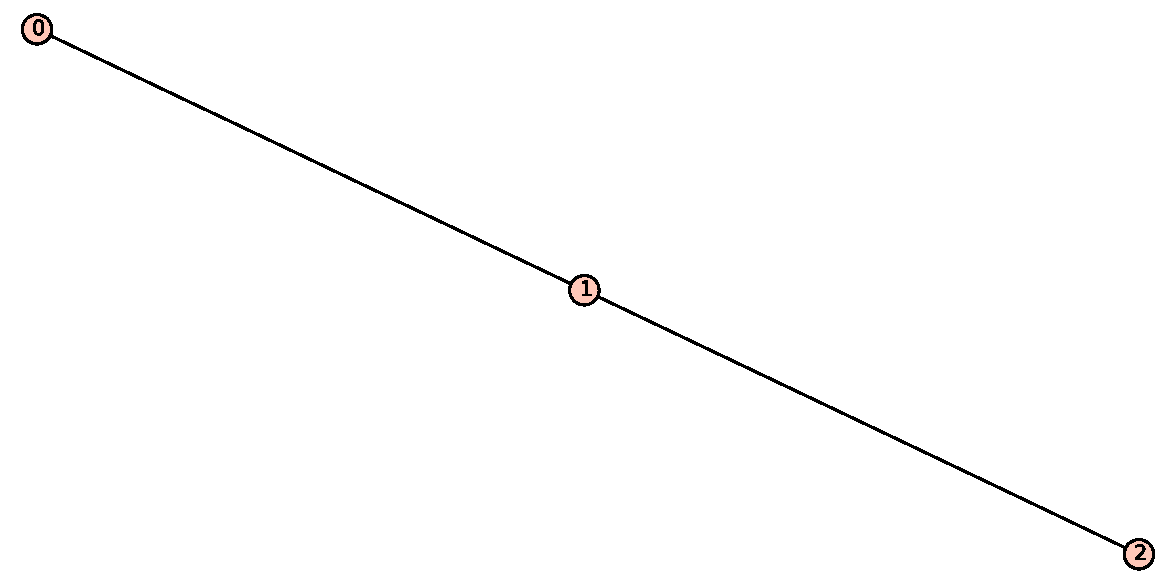
\includegraphics[scale = 0.4]{h00.pdf}
\end{center}
\caption{A graph with $V = \{0,1,2\}$ and $E = \{(0,1),(1,2)\}$.}
\label{graph}
\end{figure}
\begin{defn}We say that $u$ and $v$ are \textbf{neighbors} if
$(u,v) \in E$. 
\end{defn}
In Figure \ref{graph}, $0$ and $1$ are neighbors but
$0$ and $2$ are not neighbors. 
\begin{defn}
A \textbf{p-cycle} us a collection of $p$ distinct
vertices, $u_1,...,u_p$ such that the following properties hold:
\begin{enumerate} 
\item $(u_i,u_{i+1}) \in E, i = 1, ... , p$.
\item $(u_p,u_{1}) \in E$.
\end{enumerate} 
\end{defn}
\begin{defn} In the mathematical area of graph theory, a
\textbf{clique} in an undirected graph is a subset of its vertices such that
every two vertices in the subset are connected by an edge, i.e. $V_0$
is a clique $V_0 \subset V$ such that $\forall u \in V_0$ and $\forall
v \in V_0$, $(u,v) \in E$. $V_0$ is a \textbf{maximal clique} if 
\begin{enumerate}
\item $V_0$ is a clique
\item $\nexists \overline{V}$ such that $V_0 \subset \overline{V}
  \subset V$ and $\overline{V}$ is a clique.
\end{enumerate}
\end{defn}
In Figure \ref{cliqgraph}, \{0,1,2\} and \{1,3\} are a maximal cliques, but \{1,2\} isn't.
\begin{figure}
\begin{center}
  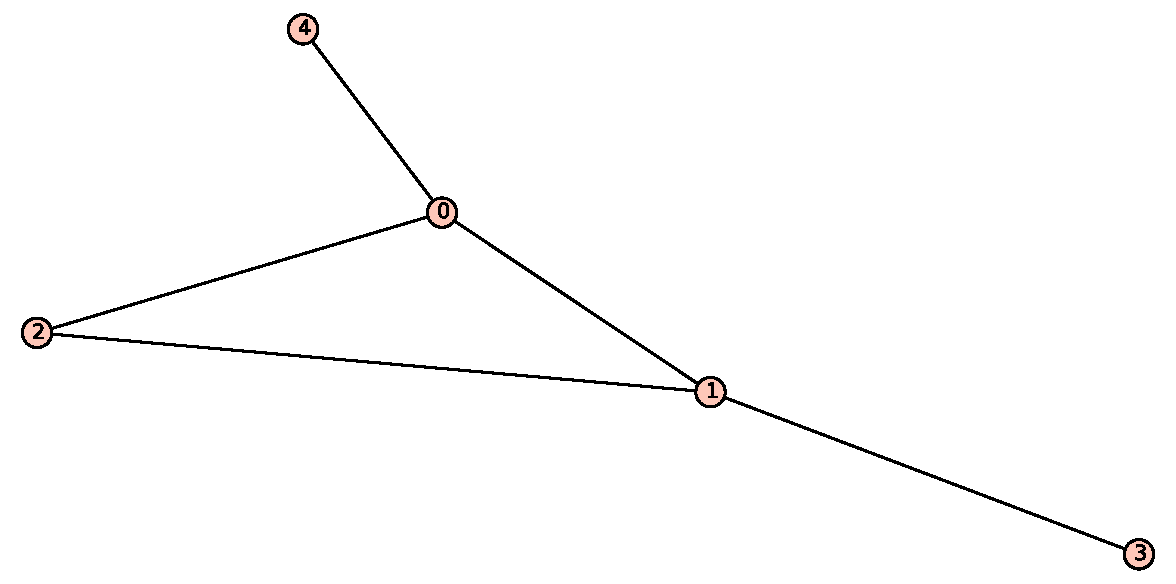
\includegraphics[scale = 0.4]{h02.pdf}
\end{center}
\caption{A graph with $V = \{0,1,2,3,4\}$ and $E = \{(0,1),(0,2),(0,4),(1,2),(1,3)\}$.}
\label{cliqgraph}
\end{figure}
\subsection{Concentration Graph Models}
Let $X^1, ... X^n \stackrel{iid}{\sim} \mathcal{N}_p (0, \s)$. We are
interested in estimating $\om = \s^{-1}$, where the $\om_{ij}$ are
restricted to be 0.
\begin{lemma}(No distributional Assumptions) Let $X \in \rp$ be
a random vector and $Cov(X) = \s = \om^{-1}$. Then $\om_{ij} =
Cov(X_i,X_j|X_k,k \neq i, k \neq j)$. 
\end{lemma}
\begin{lemma}
If we make the distributional assumption that $X \sim
\mathcal{N}_p(0,\s)$, $\om_{ij} = 0 \lra X_i|X_k \ind X_j|X_k, k
\neq i, k \neq j$.
\end{lemma}
\paragraph{Example} It makes sense to look at conditional
covariances as in many cases it turns out that variables that are
marginally dependent are conditionally independent. Consider income,
race and crime. Marginally, it seems that crime and race are dependent
but after conditioning on income, crime and race are independent.
\paragraph{Model Corresponding to Graph, $G = (V,E)$:} 
Let $\om \in \pg \coloneqq $ \{ $A| A \in \pd$ and $A_{ij} = 0$ whenever
$(i,j) \not\in E$\} and suppose that the number of elements in $V,
\abs{V} =p$. As an example consider the graph, shown in Figure \ref{omgraph},
\begin{align*}
G_1 &= (V,E), \\
\text{ where } V &= \{0,1,2,3,4\} \\
\text{ and } E &= \{(0,1),(0,2),(0,3),(1,4),(2,4)\}.
\end{align*}
Then $\om \in
\mathbb{P}_{G_1}$ and
the corresponding concentration matrix for this graph is 
\begin{align*}
\om &=  \begin{pmatrix}
\omega_{11}&\omega_{12}&\omega_{13}&\omega_{14}&0\\ 
\omega_{21}&\omega_{22}&0&0&\omega_{25}\\ 
\omega_{31}&0 &\omega_{33}&0&\omega_{35}\\ 
\omega_{41}&0&0&\omega_{45}&0\\ 
0&\omega_{52} &\omega_{53}&0&\omega_{55}
\end{pmatrix}.
\end{align*}
\begin{figure}
\begin{center}
  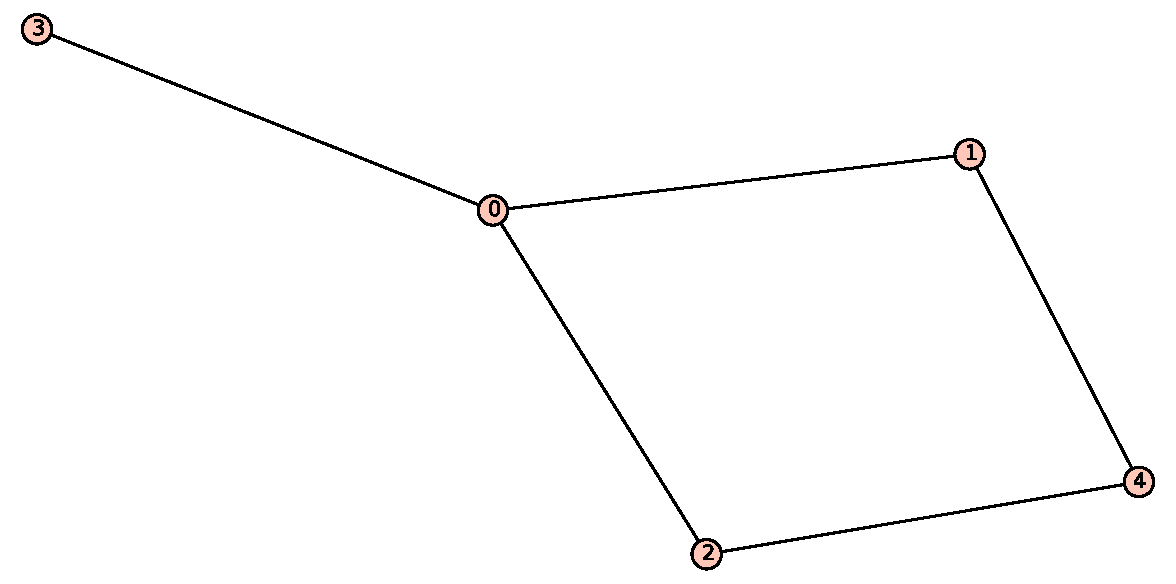
\includegraphics [scale=0.4]{h01.pdf}
\end{center}
\caption{A graph with $V = \{0,1,2,3,4\}$ and $E = \{(0,1),(0,2),(0,3),(1,4),(2,4)\}$.}
\label{omgraph}
\end{figure}
Suppose $n=2p>p$. Then $\hat{\om} = S^{-1}$ is a valid estimate as $
S^{-1}$ exists. However, we cannot put 0s into $S^{-1}$ arbitrarily
as we need to preserve the positive definite structure to have a valid
estimate. 
\begin{lemma} If $A$ is positive definite and we construct 
\begin{align*}
 A_{G} =
  \begin{cases}
   A_{ij} & \text{if } (i,j) \in E \\
   0       & \text{if } (i,j) \not\in E 
  \end{cases}
\end{align*}
Then $A$ is not positive definite in general. (Under some assumptions
$A_G$ may be positive definite asymptotically but that still doesn't
give us an estimator for a fixed $n$ and $p$.)
\end{lemma}
\subsubsection{(Negative) Log Likelihood} If $X^{1}, ... , X^{n} \sim \mathcal{N}_p(0,\Sigma =
\Omega^{-1}), G = (V,E), \abs{V} = p, \Omega \in \pg$, then the
negative log likelihood is, 
\[
l(\Omega) = c +
\frac{n}{2}tr(\om S)-\frac{n}{2}\log\abs{\Omega}
\] 
where $\Omega \in \pg$ and $c$ is a constant. $l(\om)$ has a unique
global minimum if $n> max \{\abs{C_1},...,\abs{C_n} \}$ where
$C_1,...,C_n$ denotes the cliques of $G$. 
\begin{figure}
\begin{center}
  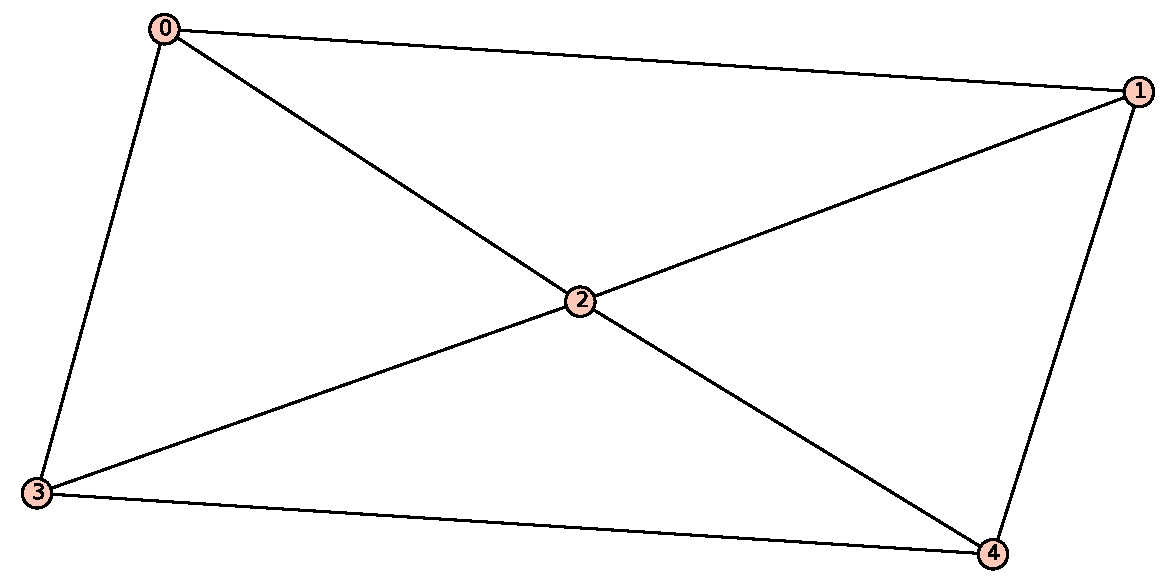
\includegraphics [scale=0.4]{h11.pdf}
\end{center}
\caption{A graph with $V = \{0,1,2,3,4\}$ and $E = \{(0,1),(0,2),(0,3),(1,2),(1,4),(2,3),(3,4)\}$.}
\label{clkgraph}
\end{figure}
In Figure \ref{clkgraph}, $p=5$ and the cliques are $C_1 = {0,1,2}$,$C_2 = {0,2,3}$,$C_3 =
{2,3,4}$,$C_4 = {1,2,4}$. Thus $max \abs{C_i} = 3$. Hence for a unique
maximum likelihood estimator to exist we need $n>3$.
Now for $\om \in \pg$, consider $\l^{*}(\om) = tr(\om S) - \log
\abs{\om}$, which has a minimum at the same $\om$ as $l(\om)$. In
general there is no closed form for the global minimum. Hence we need
to use iterative minimization techniques.
\subsubsection{Iterative Proportional Fitting (IPF)} Speed and Kiveri
(1986) came up with the following algorithm:
\begin{enumerate}
\item Start with an initial estimate $\om^{0} \in \pg$.
\item Set $\om^{(r,0)} = \om^{0}$.
\item Repeat the following for $i = 1, ..., k$ where $k$ is the number
  of cliques and the vertex set,
  $V = C_i \cup \bar{C_i}$ and $\bar{C_i} = V \setminus C_i$:
\begin{itemize}
\item Set $\om^{(r,i)} = \om^{i-1}$
\item $\om^{(r,i)} =  \arg\min \{ tr(AS) - \log \abs{A} \}$
where
\[
A: 
\begin{cases} (A^{-1})_{C_i \bar{C_i}} = \s_{C_i \bar{C_i}}^{(r,i-1)} \\
(A^{-1})_{\bar{C_i} \bar{C_i}} = \s_{\bar{C_i} \bar{C_i}}^{(r,i-1)}
\end{cases} 
\]
\end{itemize}
More details on this step below.
\item If $\norm{\om^{(r,k)} - \om^{(r,0)}} < tol$, stop. Else set
  $\om^{(r+1,0)} = \om^{(r,k)}$ and go back to Step 3.
\end{enumerate}
To minimize the function in Step 3, first we permute the rows and columns of $\s$ to get 
\begin{align*}
\s &= 
\begin{pmatrix} 
\s_{C_1 C_1} & \s_{C_1 \bar{C_1}} \\
\s_{{C_1 \bar{C_1}}} & \s_{\bar{C_1} \bar{C_1}}  
\end{pmatrix}
\end{align*} 
Then let 
\begin{align*}
\om &= \s^{-1} \\
&= \begin{pmatrix} 
\om_{11} & \om_{12}\\
\om_{21} & \om_{22}
\end{pmatrix}
\end{align*} 
where 
\begin{align*}
\om_{11} &= (\s_{C_1 C_1} - \s_{C_1 \bar{C_1}} \s_{\bar{C_1}
  \bar{C_1}}^{-1} \s_{{C_1 \bar{C_1}}})^{-1} \\
\om_{12} &= - \om_{11} \s_{C_1 \bar{C_1}} \s_{\bar{C_1}
  \bar{C_1}}^{-1} \\
\om_{21} &= - \s_{\bar{C_1}
  \bar{C_1}}^{-1} \s_{ \bar{C_1} C_1} \om_{11} \\
\om_{22} &= \s_{\bar{C_1}
  \bar{C_1}}^{-1} + \s_{\bar{C_1}
  \bar{C_1}}^{-1} \s_{C_1 \bar{C_1}}  \om_{11} \s_{{C_1
           \bar{C_1}}} \s_{\bar{C_1}
  \bar{C_1}}^{-1} 
\end{align*}
and 
\begin{align*}
S &= 
\begin{pmatrix} 
S_{C_1 C_1} & S_{C_1 \bar{C_1}} \\
S_{{\bar{C_1} {C_1}}} & S_{\bar{C_1} \bar{C_1}}  
\end{pmatrix}
\end{align*}
Therefore,
\begin{align*}
tr(\om S) &= tr (\s^{-1} S) \\
&= tr \Big( \begin{pmatrix} 
\om_{11} & \om_{12}\\
\om_{21} & \om_{22}
\end{pmatrix} \times \begin{pmatrix} 
S_{C_1 C_1} & S_{C_1 \bar{C_1}} \\
S_{{\bar{C_1} {C_1}}} & S_{\bar{C_1} \bar{C_1}}  
\end{pmatrix} \Big) \\
&= tr\Big( \begin{pmatrix} 
\om_{11}S_{C_1 C_1} + \om_{12} S_{{\bar{C_1} {C_1}}}  & \om_{11} S_{C_1 \bar{C_1}} + \om_{12} S_{{\bar{C_1} \bar{C_1}}} \\
\om_{21} S_{C_1 C_1}  + \om_{22} S_{{\bar{C_1} {C_1}}} & \om_{21} S_{C_1 \bar{C_1}} + \om_{22} S_{{\bar{C_1} \bar{C_1}}}
\end{pmatrix}\Big) \\
&= tr(\om_{11}S_{C_1 C_1} + \om_{12} S_{{\bar{C_1} {C_1}}}) +
  tr(\om_{21} S_{C_1 \bar{C_1}} + \om_{22} S_{{\bar{C_1} \bar{C_1}}})
  \\
&= tr(\om_{11}S_{C_1 C_1} + 2 \om_{12} S_{{\bar{C_1} {C_1}}} +
  \om_{22} S_{{\bar{C_1} \bar{C_1}}}) \\
&= tr(\om_{11}S_{C_1 C_1} + - 2\om_{11} \s_{C_1 \bar{C_1}} \s_{\bar{C_1}
  \bar{C_1}}^{-1} S_{{\bar{C_1} {C_1}}} +  \s_{\bar{C_1}
  \bar{C_1}}^{-1} S_{{\bar{C_1} \bar{C_1}}} \\ & \qquad + \s_{\bar{C_1}
  \bar{C_1}}^{-1} \s_{C_1 \bar{C_1}}  \om_{11} \s_{{C_1
           \bar{C_1}}} \s_{\bar{C_1}
  \bar{C_1}}^{-1}  S_{{\bar{C_1} \bar{C_1}}})
\end{align*}
Thus 
\begin{align}
tr(\om S) &= tr (\s^{-1} S) \nonumber \\
&= tr(\om_{11}S_{C_1 C_1}) + tr(-2\om_{11} \s_{C_1 \bar{C_1}} 
\s_{\bar{C_1} \bar{C_1}}^{-1} S_{{\bar{C_1} {C_1}}}) +  
tr(\s_{\bar{C_1} \bar{C_1}}^{-1} S_{{\bar{C_1} \bar{C_1}}}) \nonumber \\ 
& \qquad + tr(\s_{\bar{C_1}
  \bar{C_1}}^{-1} \s_{C_1 \bar{C_1}}  \om_{11} \s_{{C_1
           \bar{C_1}}} \s_{\bar{C_1}
  \bar{C_1}}^{-1}  S_{{\bar{C_1} \bar{C_1}}}) \nonumber \\
&= tr(\om_{11}S_{C_1 C_1}) + tr(-2\om_{11} \s_{C_1 \bar{C_1}} \s_{\bar{C_1}
  \bar{C_1}}^{-1} S_{{\bar{C_1} {C_1}}}) +  tr(\s_{\bar{C_1}
  \bar{C_1}}^{-1} S_{{\bar{C_1} \bar{C_1}}}) \nonumber \\ 
& \qquad + tr(\om_{11} \s_{{C_1
           \bar{C_1}}} \s_{\bar{C_1}
  \bar{C_1}}^{-1}  S_{{\bar{C_1} \bar{C_1}}} \s_{\bar{C_1}
  \bar{C_1}}^{-1} \s_{C_1 \bar{C_1}}) \nonumber \\
\label{eq:traceterm}
&= tr(\om_{11} (S_{C_1 C_1} -2 \s_{C_1 \bar{C_1}} \s_{\bar{C_1}
  \bar{C_1}}^{-1} S_{{\bar{C_1} {C_1}}}  
+ \s_{{C_1
           \bar{C_1}}} \s_{\bar{C_1}
  \bar{C_1}}^{-1}  S_{{\bar{C_1} \bar{C_1}}} \s_{\bar{C_1}
  \bar{C_1}}^{-1} \s_{C_1 \bar{C_1}})) \\ & \qquad +  tr(\s_{\bar{C_1}
  \bar{C_1}}^{-1} S_{{\bar{C_1} \bar{C_1}}}) \nonumber
\end{align}
For the second term: $\log \abs{\om}$, recall from Equation
\ref{eq:schurdet} that if 
\[
M = \begin{pmatrix}
A&B\\ C&D
\end{pmatrix}
\]
and $D$ is invertible, then $\abs{M} = \abs{D} \abs{A-BD^{-1}C}$. Thus,
\begin{align*}
\abs{\s} &= \abs{\s_{\bar{C_1} \bar{C_1}}}
                    \abs{\underbrace{\s_{C_1 C_1} - \s_{C_1 \bar{C_1}}
                    \s_{\bar{C_1}  \bar{C_1}}^{-1} \s_{{C_1 \bar{C_1}}}}_{\om_{11}^{-1}}}\\
&= \abs{\s_{\bar{C_1} \bar{C_1}}} \abs{\om_{11}^{-1}} \\
&= \frac{\abs{\s_{\bar{C_1} \bar{C_1}}}}{\abs{\om_{11}}} \\
\implies \log \abs{\om} &= \log \abs{\s^{-1}} \\
&= \log(\frac{1}{\abs{\s}}) \\  
& = \log \Big( \frac {\abs{\om_{11}}}{\abs{\s_{\bar{C_1} \bar{C_1}}}} \Big)\\
&= \log{\abs{\om_{11}}} - \log{\abs{\s_{\bar{C_1} \bar{C_1}}}}
\end{align*}
As $C_1$ is a clique, all the nodes in $C_1$ are connected to every
other node in $C_1$ and hence there are no 0's in $\om_{11}$. Thus
 $\om_{11}$ is positive definite with no constraints. The idea in IPF
 is to maximize $l^{*}(\om)$ over $C_1$ while hold everything else
 constant, which in this case is $\s_{{C_1} \bar{C_1}}$ and
 $\s_{\bar{C_1} \bar{C_1}}$.
\begin{align*}
l^{*}(\om) &= tr (\om S) - \log \abs{\om} \\
&= tr (\s^{-1} S) - \log \abs{\om} \\
& =  tr(\om_{11} (S_{C_1 C_1} -2 \s_{C_1 \bar{C_1}} \s_{\bar{C_1}
  \bar{C_1}}^{-1} S_{{\bar{C_1} {C_1}}}  
+ \s_{{C_1
           \bar{C_1}}} \s_{\bar{C_1}
  \bar{C_1}}^{-1}  S_{{\bar{C_1} \bar{C_1}}} \s_{\bar{C_1}
  \bar{C_1}}^{-1} \s_{C_1 \bar{C_1}})) \\ 
& \quad  + \log{\abs{\om_{11}}} + \text{terms not depending on } \om_{11}
\end{align*}
 To maximize with respect to $\om_{11}$ we can simply take the
 derivative and set it equal to 0. As $C_1$ is a clique, $S_{C_1 C_1}$
 is clearly positive definite as $n>\abs{C_1}$. It can also be shown
 that $S$ is positive definite in such a case. (Need a reference/proof
 of this fact).
\begin{lemma}If $n>max\{C_1,...C_k\}$,i.e. the sample size is bigger than the largest
clique size, then $l^{*}(\om)$ is strictly convex. 
Lauritzen(1996) has conditions for convergence of the partial
minimization algorithm under convexity of $l^{*}(\om)$. 
\end{lemma}
For non-convex
$l^{*}(\om)$ look at Drton and Elder (2006).
\begin{defn} let $G = (V,E)$ be a graph. Then $G_1
= (V_1,E_1)$ is a \textbf{subgraph} of $G$ if $V_1 \subset V$ and $E_1 \subset
E$. In addition, if $(u,v) \in E_1$ whenever $u \in V_1 \& v \in V_1$,
then $G_1$ is an \textbf{induced subgraph} of $G$. 
\end{defn}
\begin{figure}
\begin{center}
  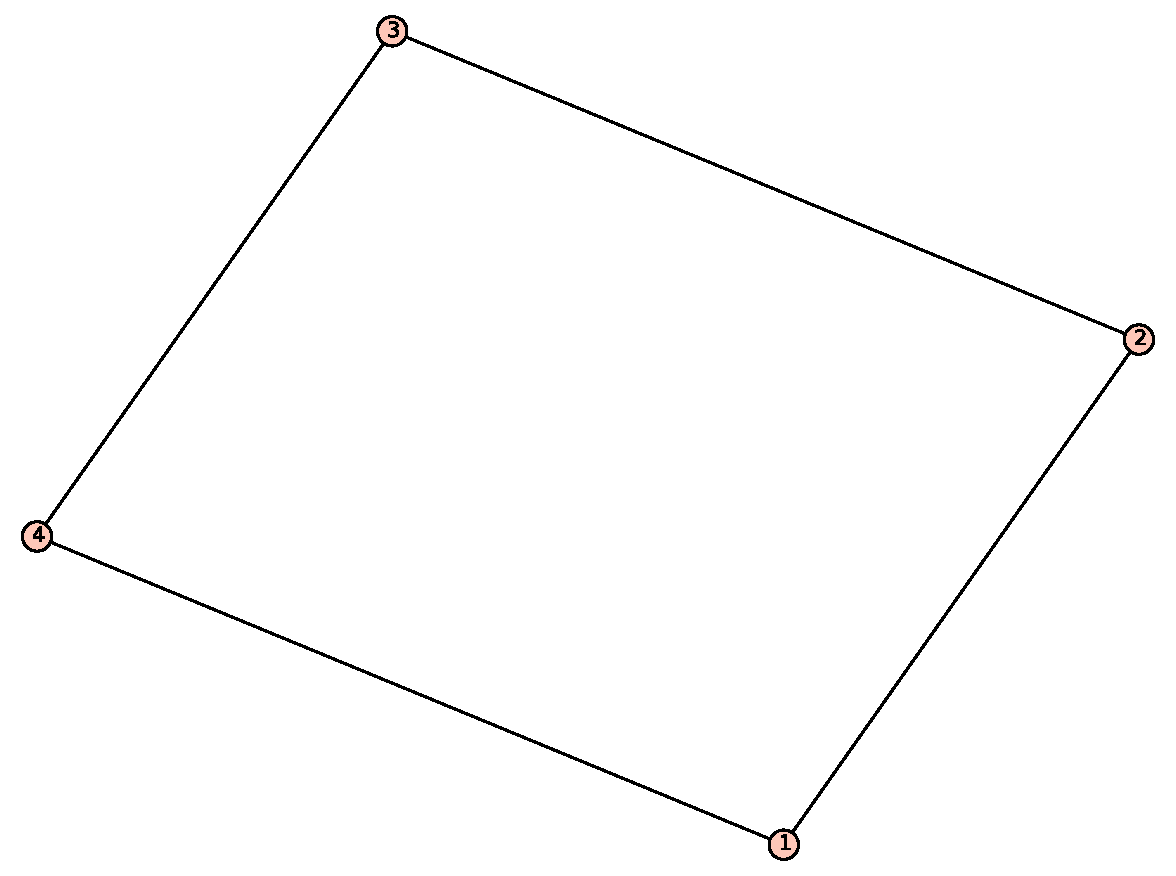
\includegraphics [scale=0.4]{h03.pdf}
\end{center}
  \caption{A graph with $V = \{1,2,3,4\}$, $E =
    \{(4,1),(1,2),(2,3),(3,4)\}$.}
\label{4cycle}
\end{figure}
\begin{figure}
\centering
\begin{subfigure}{.5\textwidth}
  \centering
  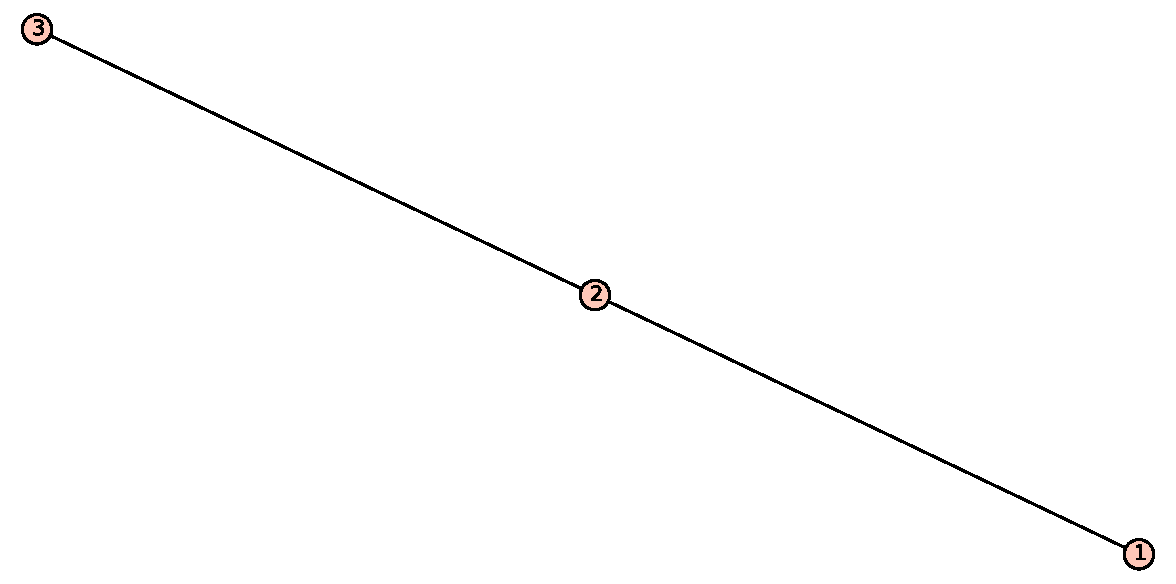
\includegraphics [scale=0.3]{h05.pdf}
\caption{An induced graph with $V_1=\{1,2,3\} \subset V$, $E_1=
    \{(2,3),(1,2)\} \subset E$.}
  \label{graph4induced}
\end{subfigure}%
\begin{subfigure}{.5\textwidth}
  \centering
  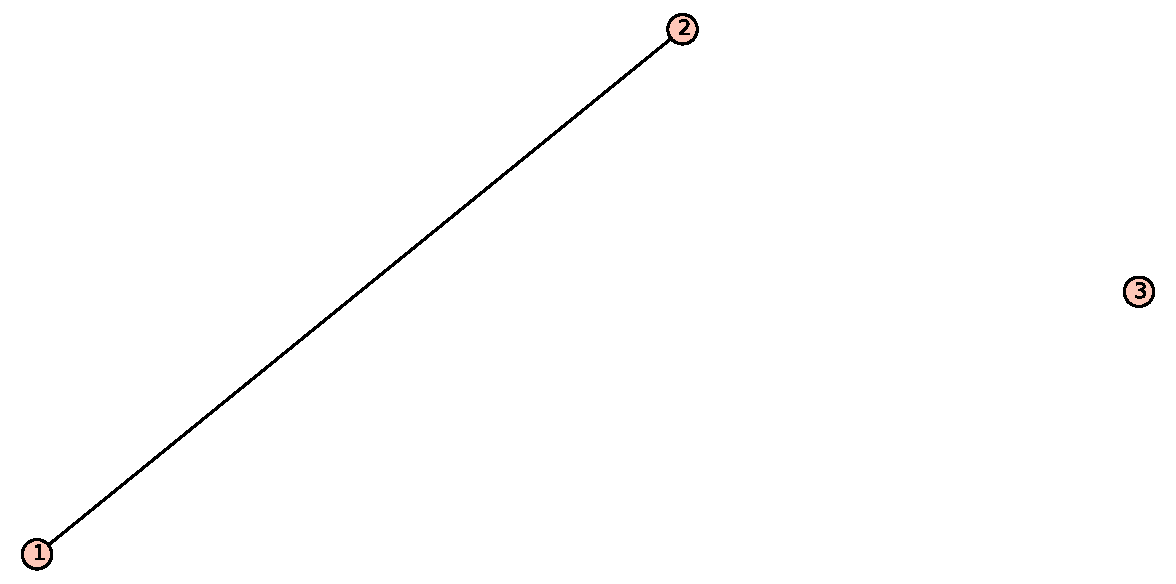
\includegraphics [scale=0.3]{h04.pdf}
  \caption{A subgraph with $V_1=\{1,2,3\} \subset V$, $E_1=
    \{(1,2)\} \subset E$.}
  \label{subgraph4v}
\end{subfigure}
\caption{Subgraphs}
\label{notinducedsubgraph}
\end{figure}
\begin{defn} (We need this concept in
Definition 2 of decomposable graphs) Let $G =
(V,E)$ be a graph. An \textbf{ordering of the vertices} is a bijection,$\sigma
$ from $V$ to the set $\{1,2,...,\abs{V}\}$. Then the \textbf{ordered graph}
$G_{\sigma} = (V_{\sigma} ,E_{\sigma} )$ where $V_{\sigma} =
\{1,2,...,\abs{V}\}$ and $(i,j) \in E_{\sigma} \iff
(\sigma^{-1}(i),\sigma^{-1}(j)) \in E$. An ordering $\sigma$ is
defined to be a \textbf{perfect elimination ordering} if $\not\exists  i>j>k$
such that $(i,j) \not\in E_{\sigma}$ but $(j,k) \in  E_{\sigma}$ and
$(i,k) \in E_{\sigma}$. 
\end{defn}
Consider the graph in Figure
\ref{graph4induced}. If 
\begin{align*}
\sigma_1 = \begin{pmatrix} 0 &1 & 2 \\
2 & 1 & 3 \\
\end{pmatrix}
\end{align*}
then $3>2>1$ and $(2,3) \not\in  E_{\sigma}$ but $(2,1) \in
E_{\sigma}$ and $(3,1) \in  E_{\sigma}$.
Thus $\sigma_1$ is not a perfect elimination ordering. However,
\begin{align*}
\sigma_2 = \begin{pmatrix} 0 &1 & 2 \\
2 & 3 & 1 \\
\end{pmatrix}
\end{align*}
is a perfect elimination ordering scheme.
\begin{figure}
\centering
\begin{subfigure}{.5\textwidth}
  \centering
  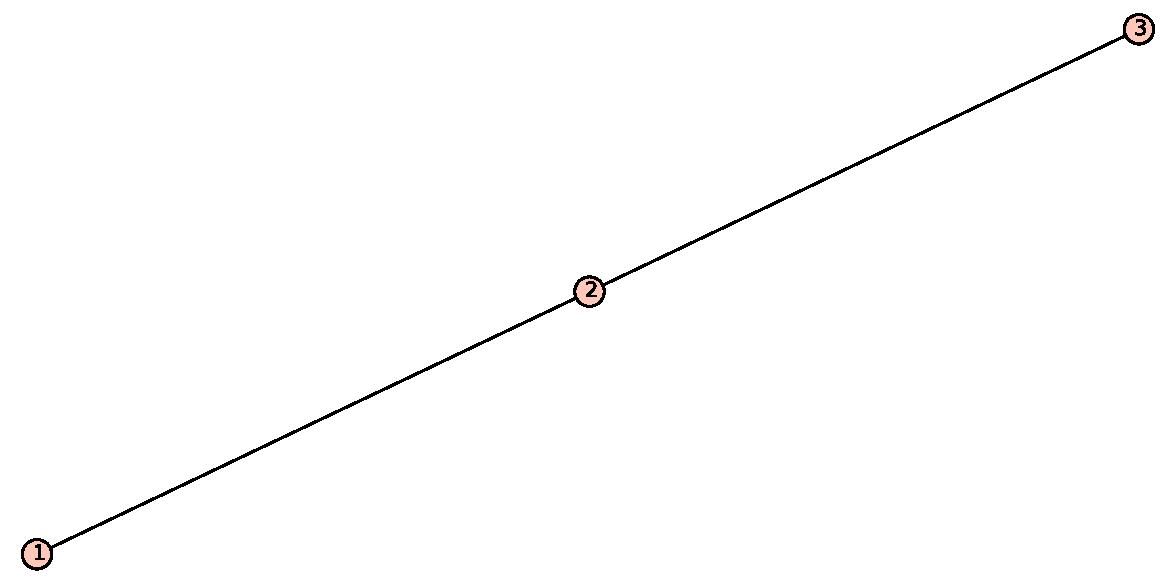
\includegraphics [scale=0.3]{h07.pdf}
\caption{Not a perfect elimination ordering of the vertices}
  \label{notperfect}
\end{subfigure}%
\begin{subfigure}{.5\textwidth}
  \centering
  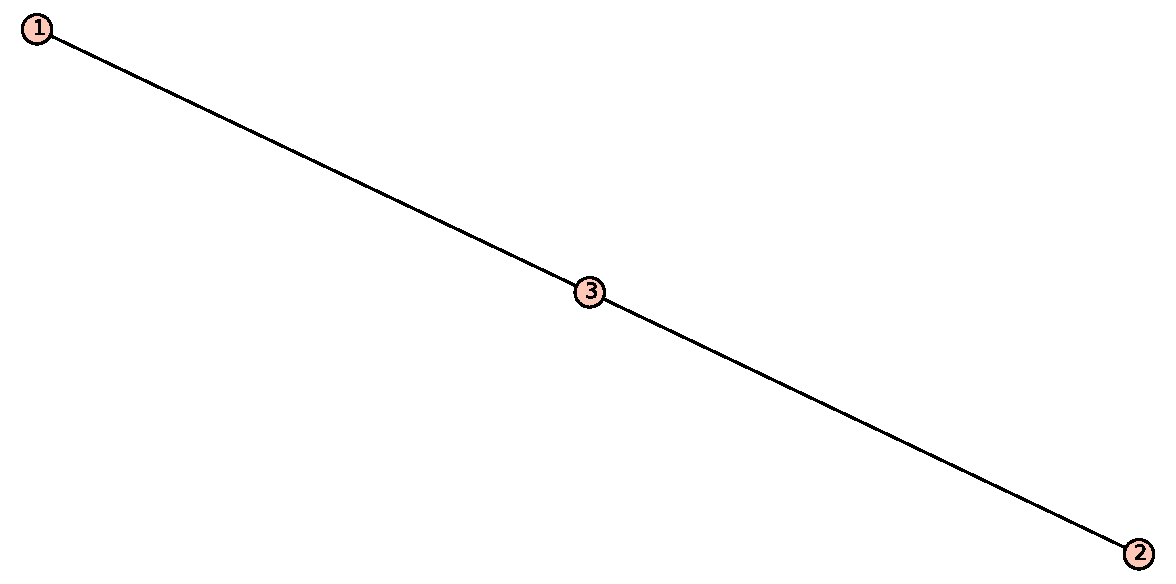
\includegraphics [scale=0.3]{h08.pdf}
  \caption{A perfect elimination ordering of the vertices}
  \label{perfect}
\end{subfigure}
\caption{Perfect Elimination Orderings}
\label{Perfectorder}
\end{figure}
\begin{defn} (We need this concept in
Definition 3 of decomposable graphs.) If $\om$ is a positive definite
matrix, then $\exists$ a unique pair $(L,D)$ such that
\begin{enumerate}
\item $\om = LDL^T$ is the \textbf{modified Cholesky decomposition} of $\om$
\item $L$ is a lower triangular matrix with 1's on the diagonals 
\item $D$ is a postive diagonal matrix (i.e. $d_{ii}>0 \forall i$)
\end{enumerate}
\end{defn}
\subsubsection{Decomposable graphs} There are many equivalent
definitions of decomposable graphs.
\begin{defn}A graph $G=(V,E)$ is \textbf{decomposable} if and
only if it does not contain a cycle of length greater than equal to 4.
\end{defn}
Figure \ref{4cycle} is not decomposable, but Figure \ref{decomp4} is.
\begin{figure}
\begin{center}
  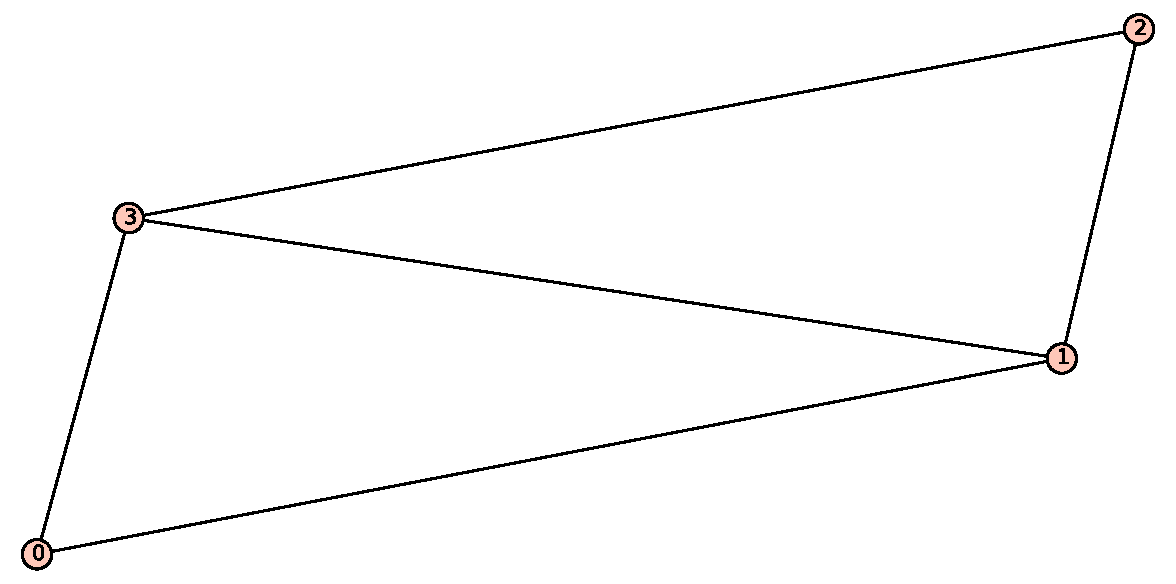
\includegraphics [scale=0.4]{h06.pdf}
\end{center}
  \caption{A graph with $V = \{0,1,2,3\}$, $E =
    \{(0,1),(0,3),(1,2),(1,3),(2,3)\}$.}
\label{decomp4}
\end{figure}
\begin{defn}A graph is \textbf{decomposable} if and only if it
has a perfect elimination ordering. Thus if we can find a perfect
elimination ordering then it means that the graph is decomposable. 
\end{defn}
\begin{defn}
\label{defn:decompldl}
A graph $G = (V,E)$ is \textbf{decomposable} if and only if there exists
and ordering, $\sigma$, of the vertices such that if $\s = LDL^T$ is the modified
Cholesky decomposition corresponding to this ordering, then for $i>j,
L_{ij} = 0 \iff \s_{ij} = 0 \iff (i,j) \not\in E_{\sigma}$. Note that
the order is of utmost importance due to uniqueness. If the order is
changed, then we get a new Cholesky decomposition. 
\end{defn}
\begin{defn}A graph is \textbf{decomposable} if and only if there
is no chorldless cycle of length greater than or equal to 4 as an
induced subgraph.
\end{defn} 
\begin{defn}
\label{defn:prfctordrmxcliqs}
Let $G = (V,E)$ be a decomposable graph. Then there exists an ordering
of the maximal cliques $C_1, ... , C_k$ such that for every $2 \leq j
\leq k$
\[
R_j = C_j \cap (\cup_{l = 1}^{j-1} C_l)
\]
\begin{enumerate}
\item $R_j \subset C_i\ text{ for some } 1 \leq i \leq j-1$.
\item $R_j$ is called the j-th \textbf{minimal separator} 
\end{enumerate}
\end{defn}
The above definition simply states that we can order the cliques so
that for any clique, say $C_h$, in that given ordering we can find some previous
clique,$C_i, 1 \leq i \leq h$, that contains the intersection of the
the clique, $C_h$ with all previous cliques, $C_1,...,C_{h-1}$.
\subsubsection{Iterative Partial Minimization(IPM)} We first consider
coordinate wise minimization, which is a special case of IPM. Suppose we are interested in minimizing a
function, $f(x), x = (x_1,...,x_p) \in \mathcal{X}$. Note that $x \mapsto (x_i,x_{-i})$ is a
bijection. Coordinate-wise
minimization consists of repeating the following steps for $i = 1,
... , p$
\begin{enumerate}
\item Minimize $f$ with respect to $x_i$ holding the other blocks constant. 
\end{enumerate}
In IPM our main objective is to minimize $f(x),x \in
\mathcal{X}$. Let $x \mapsto (y^i,y^{-i})$ be a bijection. For
example, let $x = (x_1,x_2)$, $y^{i} = x_1+x_2$ and $y^{-i} =
x_1-x_2$. Then $x \mapsto (y^i,y^{-i})$ is a bijection as given any
$x$ we can find $y^i$ and $y^{-i}$ and vice versa. Now, the main idea
of IPM is to minimize $f$ with respect to $y^i$ holding $y^{-i}$
constant, and then with respect to $y^{-i}$ holding $y^i$
constant. 
Recall that in IPF our
goal is to minimize $l^{*}(\om)$. Earlier we had mentioned that IPF is
a special case of IPM. Consider partitioning $\om$ in the following manner: 
\[
\om = \begin{pmatrix} \om_{11} & \om_{12} \\
\om_{21}& \om_{22} \\
\end{pmatrix}
\]
Now $\om_{12} = \om_{21}'$, thus $\om \mapsto
(\om_{11},(\om_{21},\om_{22}))$ is a bijection. Thus according to IPM
maximizing over $\om_{11}$ holding $(\om_{21},\om_{22})$ constant and
then maximizing over $(\om_{21},\om_{22})$ while holding $\om_{11}$
constant would be a valid approach. However, ensuring positive
definiteness of $\om$ is difficult if we approach the problem in this
manner. As a result we consider the bijection: $\om \mapsto (\om_{11}
- \om_{12} \om_{22}^{-1} \om_{21},(\om_{21},\om_{22}))$.  
\begin{thm} (Iterated Partial Maximization) If
\begin{enumerate}
\item $L:\Theta \to \mathbb{R}$ is continuous and $\Theta$ is compact
\item $\forall \theta^* \in \Theta,\exists$
  section,$\Theta_i(\theta^*), i = 1,...,k$ in $\Theta$ in such a way
  that $L$ is globally maximized at $\theta^*$ if and only if $L$ is
  maximized over all of the sections.
\item The operations of maximizing $L$ over the sections is continuous
  and well defined, i.e. there are continuous transformations $T_i$ of
  $\Theta$ into itself such that if $\theta \in \Theta_i(\theta^*)$
  for $i = 1,...,k$
\[
L\{T_i(\theta^*)\} > L(\theta), \quad \theta \not=T_i(\theta^*)
\]
In other words $T_i(\theta^*)$ is the uniquely determined point where
L is maximized over the section $\Theta_i(\theta^*)$.
Now let $\theta_0$ be arbitrary and define recursively 
\[
\theta_{n+1} = T_1 ... T_k (\theta_n), \quad n \geq 0.
\]
\item $L(\theta)$ is uniquely maximized at $\hat{\theta}$.
\end{enumerate}
Then $\theta_n \to \hat{\theta}$.
\end{thm}
\begin{proof} Since $\Theta$ is compact, the sequence $(\theta_n)$
has a convergent subsequence $(\theta_{n_l})$ such that as $l \to
\infty$, $(\theta_{n_l}) \to \theta^* \in \Theta$. We need to show
that $\hat{\theta} = \theta^*$.  Let $S = T_1 ... T_k$, that is,
$\theta_{n+1} = S (\theta_n)$. Since each $T$-operation is a partial
maximization, that is $L\{T_i(\theta^*)\} > L(\theta), \forall \theta \not=T_i(\theta^*)
$ , $L(\theta_n)$ must be non-decreasing in $n$. Thus $n+1>n
\implies L(\theta_{n+1}) \geq L(\theta_{n})$. Hence as $n_{l+1} \geq
n_l + 1 > n_l$
we have $L(\theta_{n_{l+1}}) \geq L(\theta_{n_{l}})$. Also, limits are
preserved by continuity. Thus,
\begin{align*}
L\{S(\theta^*)\} &= \lim_{l\to\infty} L\{S(\theta_{n_l})\} \quad
                   \text{by 1,2 and } l \to
\infty,(\theta_{n_l}) \to \theta^* \in \Theta \\
&\leq \lim_{l\to\infty} L(\theta_{n_{l+1}}) \\
&= L(\theta^*) \\ 
&\leq L\{T_k(\theta^*)\} \quad \text{as each $T_i$ is a partial
  maximization}\\
&\quad \vdots \\
&\leq L\{T_1 ... T_k(\theta^*)\}\\
&\leq L\{S(\theta^*)\}
\end{align*}
Thus there must be equality at every step. As the partial maxima are
unique, we also have that 
\[
\theta^* = T_k(\theta^*) = ... = T_1(\theta^*). 
\]
Finally since the global maximum was uniquely determined by maximizing
$L$ over all sections, the proof is complete. 
\end{proof}
\subsubsection{Application of IPM to maximizing $l^{*}(\om)$} Let
\begin{align*}
X^1, ... X^n &\distas{iid} \mathcal{N}_p(0, \s = \om^{-1})\\ 
\om \in \pg &= \{A \in \pd|A_{ij} = 0 \iff (i,j)\not\in E \} \\
\pd &= \{ p \times p \text{ positive definite matices }\} \\
\mathcal{L}_G &= \{L|L \text{ is lower triangular}; \\
&\quad \quad \quad L_{ii} = 1
  \forall i = 1,...p; \\
&\quad \quad \quad i>j,(i,j)\not\in E \implies L_{ij} = 0\} \\
\mathcal{D} &= \{D| D \text{ is diagonal with} D_{ii}>0 \}
\end{align*}
\begin{figure}
\begin{center}
  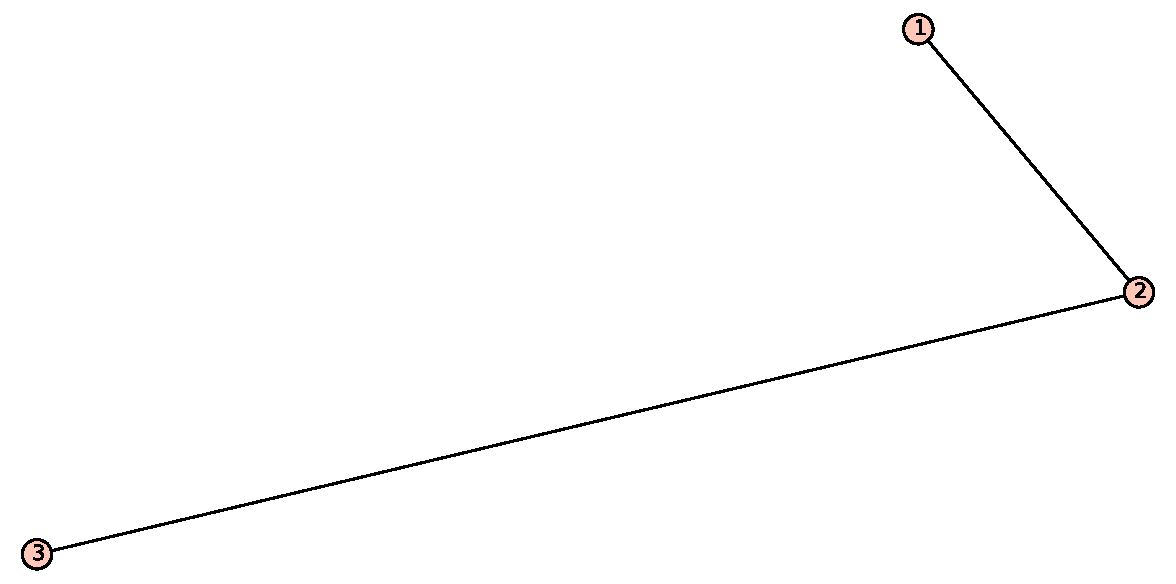
\includegraphics [scale=0.4]{h10.pdf}
\end{center}
  \caption{A graph with $V = \{1,2,3\}$, $E =
    \{(1,2),(2,3)\}$.}
\label{cholgraph}
\end{figure}
Consider the graph in Figure \ref{cholgraph}. The corresponding $L \in
\mathcal{L}_G$ is
\[
L = 
\begin{pmatrix} 1&0&0\\
l_{21}&1&0\\
0&l_{32}&0\\
\end{pmatrix}
\]
where $l_{31} = 0$ as $(3,1) \not\in E$. Now recall that from Definition
\ref{defn:decompldl} that $G$ is decomposable if and only if there is
a perfect vertex elimination scheme if and only if the ordering of
the vertices for that perfect
vertex elimination scheme implies $\om = LDL^T$ and $(i,j) \not\in E \implies
L_{ij} = 0$. In addition, $\om \mapsto (L,D)$ such that $\om = LDL^T$
is a bijection from $\pg$ to $\mathcal{L}_G \times \mathcal{D}$. This is
because, once an ordering of the vertices has been fixed, the cholesky
decomposition is unique. In general, a positive definite matrix has a
unique cholesky decomposition, but there may be several perfect
elimination orderings. Thus given and $\om$ we can find a unique $L$
and a unique $D$ and vice versa. As a result, using the concepts from IPM, to minimize $l^*(\om)$ we
can minimize $l^*(L,D)$ instead. Note that 
\begin{align*}
l^*(\om) &= tr(\om S) - \log \abs{\om} \\
\implies l^*(L,D) &= tr(LDL^T S) - \log \abs{LDL^T} \\
&= tr(DL^T SL) \quad \{tr(AB) = tr(BA)\}\\
&\qquad - \log \abs{L} \abs{D} \abs{L^T} \quad \{det(ABC) = det(A)
  det(B) det(C) \} \\
&= tr(DL^T SL) - \log \abs{D} \quad \{det(L) = \prod_{i=1}^p L_{ii} =
  1 \} \\
&= tr(DL^T SL) - \log \prod_{I=1}^p D_{ii} \quad \{det(D) = \prod_{i=1}^p D_{ii} =
  1 \} \\
&= \sum_{i=1}^p (D_{ii}(L_{.i}^TSL_{.i})-log D_{ii})
\end{align*}
In the final step we have used the following facts
\begin{enumerate} 
\item Pre-multiplying a matrix
\begin{align*}
A = \begin{pmatrix} 
a_{11} & a_{12} & \hdots & a_{1p} \\
a_{21} &a_{22} & \hdots&  a_{2p} \\
\vdots & \vdots &\ddots& \vdots\\
a_{p1} &a_{p2} & \hdots & a_{pp} 
\end{pmatrix}
\end{align*}
by a diagonal matrix 
\begin{align*}
D = \begin{pmatrix} 
d_{11} & 0 & \hdots & 0 \\
0 &d_{22} & \hdots&  0 \\
\vdots & \vdots &\ddots& \vdots\\
0 &0 & \hdots & d_{pp} 
\end{pmatrix}
\end{align*}
leads to multiplying the $i$-th row of $A$ by $d_{ii}$, i.e.
\begin{align*}
AD = \begin{pmatrix} d_{11} a_{11} & d_{11} a_{12} & \hdots & d_{11} a_{1p} \\
d_{22} a_{21} &d_{22} a_{22} & \hdots&  d_{22} a_{2p} \\
\vdots & \vdots &\ddots& \vdots\\
d_{pp}  a_{p1} &d_{pp}  a_{p2} & \hdots &d_{pp}  a_{pp} 
\end{pmatrix}
\end{align*}
\item $(SL)_{ij} = S_{i.}L_{.j} \implies (SL)_{.j} = S L_{.j} $ 
\begin{align*}
(SL)_{1j} &= S_{1.}L_{.j} \\
(SL)_{2j} &= S_{2.}L_{.j} \\
&\hdots \\
(SL)_{pj} &= S_{p.}L_{.j} \\
\end{align*}
\item The $ii$-th entry of $L^T SL$:
 \[
(L^T SL)_{ii}  = (L^T)_{i.} (SL)_{.i} = (L_{.i})^T S L_{.i}
\]
\end{enumerate}
Now note that for each $i$ we can minimize each term in the sum
independently of $j \not= i, j = 1,...,p$. For example, if $i = 1$, we
can minimize, $(D_{11}(L_{.1}^TSL_{.1})-\log D_{11}$ and then move on
to $i = 2$. In this regard note that
\begin{align}
\label{eq:cholmin}
L_{.i}^TSL_{.i} = \begin{pmatrix} 1 & x_i^T \\
\end{pmatrix}
\begin{pmatrix} S_{ii} & S_{.i}^> \\
S_{.i}^> & S^{>i} \\
\end{pmatrix}
\begin{pmatrix} 1 \\ x_i
\end{pmatrix}
\end{align}
where
\begin{itemize}
\item $x_i = (L)_{ji}, j>i ,(i,j) \in E$, i.e. the elements of
the $i$-th columns of $L$ that lie below the diagonal such that there is an edge between $i$ and $j$.
\item $S^{>i} = (S_{jk})_{j,k>i},(i,j) \in E,(i,k) \in E$, i.e. the submatrix of $S$ from
  the $(i+1)$-th row and $(i+1)$-th column through to the $p$-th row and $p$-th column
 such that there is an edge between $i$ and $j$ and $i$ and $k$.
\item $S_{.i}^>  = (S_{ji})_{j>i},(i,j) \in E$, i.e. the vector from
  the $i$-th column of $S$ that lie below the diagonal, $S_{ii}$
 such that there is an edge between $i$ and $j$.
\end{itemize}
For each $i = 1,...p$, first we minimize Equation \ref{eq:cholmin} with respect to $x_i$. The
solution turns out to be 
\[
\hat{x}_i = -(S^{>i})^{-1} S_{.i}^>. 
\]
Then we minimize $(D_{ii}(S_{ii} -  (S_{.i}^>)^{T} (S^{>i})^{-1} (S_{.i}^>))-\log D_{ii}$ with respect
to $D_{ii}$. This turns out to be
\[
\hat{D}_{ii} = \frac{1}{S_{ii} -  (S_{.i}^>)^{T} (S^{>i})^{-1} (S_{.i}^>)}.
\]
Then we can estimate $\om$ using
\begin{align}
\label{eq:omegahatgeneral}
\hat{\om} = \hat{L} \hat{D} \hat{L}^T
\end{align}
Now suppose that $C_1,...,C_k$ is and ordering of the maximal cliques
of $G = (V,E)$ and let $R_2,...,R_k$ be the minimal separators as in Definiton
\ref{defn:prfctordrmxcliqs}. Then 
\begin{align}
\label{eq:omegahatclosed}
\hat{\om} = \sum_{i = 1}^k [(S_{C_i})^{-1}]^0 - \sum_{i = 2}^k [(S_{R_i})^{-1}]^0
\end{align}
where for $A \subset V$
\begin{align*}
 ([(S_{A})^{-1}]^0)_{kl} =  \begin{cases} S_A^{-1} \quad \text{if }
   k \in A, l \in A\\
0 \quad \text{if } k \not\in A \text{ or } l \not\in A  
\end{cases}
\end{align*}
\paragraph{Example:}
Let 
\begin{align*}
\om &= \begin{pmatrix}{}
  0.80 & 0.37 & 0.00 & 0.31 \\ 
  0.37 & 1.37 & 0.58 & 0.39 \\ 
  0.00 & 0.58 & 0.32 & 0.16 \\ 
  0.31 & 0.39 & 0.16 & 0.69 \\ 
  \end{pmatrix}\\
\end{align*}
For simplicity suppose we have an exact estimate of $S$:
\[
 S =\om^{-1} = \begin{pmatrix}{}
  3.33 & -3.57 & 7.05 & -1.10 \\ 
  -3.57 & 7.18 & -13.36 & 0.62 \\ 
  7.05 & -13.36 & 28.52 & -2.19 \\ 
  -1.10 & 0.62 & -2.19 & 2.09 \\ 
  \end{pmatrix}
\]
Then
\[
S_{C_1} = \begin{pmatrix}{}
  3.33 & -3.57 & -1.10 \\ 
  -3.57 & 7.18 & 0.62 \\ 
  -1.10 & 0.62 & 2.09 \\ 
  \end{pmatrix} 
\text{ and } (S_{C_1})^{-1} =
\begin{pmatrix}{}
  0.80 & 0.37 & 0.31 \\ 
  0.37 & 0.32 & 0.10 \\ 
  0.31 & 0.10 & 0.61 \\ 
  \end{pmatrix}
\]
which implies that
\[
[(S_{C_1})^{-1}]^0 =
\begin{pmatrix}{}
  0.80 & 0.37 & 0.00 & 0.31 \\ 
  0.37 & 0.32 & 0.00 & 0.10 \\ 
  0.00 & 0.00 & 0.00 & 0.00 \\ 
  0.31 & 0.10 & 0.00 & 0.61 \\ 
  \end{pmatrix}. 
\]
Similarly 
\[
\implies [(S_{C_2})^{-1}]^0 = \begin{pmatrix}{}
  0.00 & 0.00 & 0.00 & 0.00 \\ 
  0.00 & 1.19 & 0.58 & 0.25 \\ 
  0.00 & 0.58 & 0.32 & 0.16 \\ 
  0.00 & 0.25 & 0.16 & 0.57 \\ 
  \end{pmatrix}
\]
and
\[
[(S_{R_2})^{-1}]^0 = \begin{pmatrix}{}
  0.00 & 0.00 & 0.00 & 0.00 \\ 
  0.00 & 0.14 & 0.00 & -0.04 \\ 
  0.00 & 0.00 & 0.00 & 0.00 \\ 
  0.00 & -0.04 & 0.00 & 0.49 \\ 
  \end{pmatrix}.
\]
Finally,
\[
\hat{\om} = [(S_{C_1})^{-1}]^0 + [(S_{C_2})^{-1}]^0 -
[(S_{R_2})^{-1}]^0  = \om.
\]
\subsubsection{Bayesian Inference for Concentration Graph Models} Let 
\[
f_{\theta}(x) = e^{x'\theta -\kappa (\theta)}h(x)
\]
where $\theta \in \tilde{\Theta} \subset \mathbb{R}^d$.
Let $\tilde{\pi}_{n_0,_x0}(\theta)$ denote a family of prior
distributions for the natural parameter $\theta$ with $n_0 \in
\mathbb{R},x_0 \in \mathbb{R}^d$ given by
\[
\tilde{\pi}_{n_0,_x0}(\theta) = e^{n_0x_0' \theta - n_0 \kappa (\theta) }.
\] 
 If $\tilde{\pi}_{n_0,x_0}(\theta)$ can be normalized to define a
 valid probability distribution say $\pi_{n_0,x_0} (\theta) $, then it
 is a valid \textbf{conjugate prior} to the Natural Exponential Family
 (NEF).
\begin{lemma}
\label{lemma:NEFposterior}
Furthermore, if $X_1,...X_n \distas{iid} f_\theta(x), \theta \in
\tilde{\Theta}$, then 
\begin{enumerate}
\item The \textbf{posterior density} is given by
  $\pi_{n_0+n,\frac{n_0 x_0+n\bar{X}}{n_0+n}} (\theta)$
\item The \textbf{posterior expectation} of $\frac{\partial \kappa
    (\theta)}{\partial \theta}$, $\E[\frac{\partial \kappa
    (\theta)}{\partial \theta}|X_1,...,X_n] =
  \frac{n_0 x_0+n\bar{X}}{n_0+n}$.
\item If, in addition, $\pi( \theta )$ is any prior such that it is
  not concentrated at a single point and, $\E[\frac{\partial \kappa
    (\theta)}{\partial \theta}|X] = aX+b$ for some constants $a,b$,
 then $a \not= 0$ and the density is necessarily of the form 
\[
\pi (\theta) = ce^{\frac{1}{a}b \theta - \frac{1}{a}(1-a) \kappa
(\theta)}
\]
In other words, it is a Diaconis-Ylvisaker(DY) prior.
\end{enumerate}
\end{lemma}
\paragraph{Example} Suppose $X_1,...X_n \distas{iid} \mathcal{N}_p(0, \s), \s =
\om^{-1} \text{ and } \om \distas{} \mathcal{W}_p (m,
\Lambda_0^{-1})$. Thus, 
\[
f(\om) \propto e^{-\frac{1}{2}tr(\Lambda_0 \om)
+ \frac{m-p-1}{2} \log \abs{\om}}
\]
Now $nS = \sum_{i=1}^{n} X_i X_i^T \sim \mathcal{W}_p(n,
\s )$. Keeping only the terms containing $\om$ implies that 
\begin{align*}
f(nS) &\propto e^{-\frac{1}{2}tr(\s^{-1} nS)
+ \frac{n}{2} \log \abs{\s^{-1}}}\\
&= e^{-\frac{1}{2}tr(\om nS)
+ \frac{n}{2} \log \abs{\om}}\\
\implies f(\om|S) &\propto e^{-\frac{1}{2}tr(\Lambda_0 \om)
+ \frac{m-p-1}{2} \log \abs{\om}-\frac{1}{2}tr(\om nS)
+ \frac{n}{2} \log \abs{\om}} \\
&= e^{-\frac{1}{2}tr(\om(\Lambda_0+nS))+\frac{m+n-p-1}{2}\log\abs{\om}}
\end{align*}
and by Lemma \ref{lemma:NEFposterior} take $\pi_{n_0,x_0} (\theta) = \mathcal{W}_p (m,
\Lambda_0^{-1})$ where $n_0 = m-p-1$ and $x_0 = \frac{\Lambda_0}{m-p-1}$, then $n_0+n = m+n-p-1$ and $\frac{n_0
  x_0+n\bar{X}}{n_0+n} = \frac{\Lambda_0+ nS}{m+n-p-1}$ or directly, 
\begin{align*}
\om|S &\distas{}
\mathcal{W}_p(n+m, (nS + \Lambda_0)^{-1})\\
\E[\s] &= \E[\om^{-1}] = \frac{\Lambda_0}{m-p-1}\\
\text{and } \E[\s|S] &= \E[\om^{-1}|S] = \frac{nS+\Lambda_0}{n+m-p-1}
\end{align*}
\subsubsection{The G-Wishart distribution}Now suppose $X^1, ... X^n \distas{iid} \mathcal{N}_p (0,
\om^{-1})$. Then 
\[
l(\om) = {-\frac{n}{2}tr(\om S)+\frac{n}{2} \log \abs{\om}}
\]
 where $\om \in \pg$. 
A problem that could arise with $\om \in \pg$ is that all the nice
properties of natural exponential families when $\om \in \pd$ may not
be retained. If $\om \in \pd$, then it is a natural exponential family
, but restricting some of the entries to $0$ could possibly violate the
properties of NEFs. Fortunately, restricting some of the entries to
be 0 does not affect the properties. If $\om \in \pg$, then 
\begin{align*}
tr(\om
S) &= \sum_{i=1}^p \sum_{j=1}^p \om_{ij}S_{ij} =
\sum_{(i,j) \in E}\om_{ij}S_{ij} +\sum_{i=j}\om_{ij}S_{ij} \\
\implies l(\om) &= ce^{-\frac{n}{2}\sum_{i=1}^p \sum_{j=1}^p \om_{ij}S_{ij}+\frac{n}{2} \log \abs{\om}}
\end{align*}
One choice of prior for $\om$ could be:
\[
\tilde{\pi}_{n_0,\Lambda}(\om) = e^{\frac{n_0}{2}tr(\om
  \Lambda)+\frac{n_0}{2} \log \abs{\om}}
\]
where $\om \in \pg, \Lambda \in \pd, n_0 > 0 \text{ not necessarily an
  integer}$. This is the kernel of the Wishart
distribution. We can generalize this to the DY class of prior
densities for $\om$ called G-Wishart with parameters $U_{p \times p} \in \pd, \delta>0$. It's
density proportional is to:
\[
\mathcal{GW}_p(\delta, U) \propto e^{-\frac{1}{2}tr(\om U) +
  \frac{\delta}{2} \log \abs{\om}}
\].
In such a case, the posterior of $\om|X^1,...,X^n \distas{} \mathcal{G}(n+\delta, S+U)$.
Letac-Massam(2007) extends the G-Wishart priors for decomposable
graphs. 
Note that if $K(\om) = \log \abs{\om}$, then $\nabla K(\om) =
\frac{1}{\abs{\om}} \times \abs{\om} \times (\om^{-1})^T = \om^{-1} =
\s$. Thus by Lemma \ref{lemma:NEFposterior}, $\E[\nabla K(\om)|X^1,...X^n] =
\E[\s|X^1,...X^n] = \frac{n_0 x_0+n\bar{X}}{n_0+n}$.
\subsubsection{Sampling from the G-Wishart if G is decomposable}
Suppose G is decomposable. Thus there is at least one perfect vertex
elimination scheme. Further suppose that the vertices have been
ordered according to this scheme. Then there exists a unique modified
cholesky decomposition, $\om = LDL^T$, which is a bijection from $\pg
\mapsto \mathcal{L}_G \times \mathcal{D}$. Given that 
\[
\pi_{\delta,U}(\om) \propto e^{-\frac{1}{2}tr(\om U) +
  \frac{\delta}{2} \log \abs{\om}}
\]
we want to find $\pi_{\delta,U} (L,D) = \pi_{\delta,U} (\om(L,D))
\abs{\frac{\partial \om}{\partial (L,D)}}$. Let us consider $p = 3$ to
see what's going on. 
\begin{align*}
\om = \begin{pmatrix} \om_{11} & \om_{12} & \om_{13}\\
\om_{21}& \om_{22} &  \om_{23} \\
\om_{31}& \om_{32} &  \om_{33} \\
\end{pmatrix}
\end{align*} 
where $\om_{ij} = \om_{ji}$ and
\begin{align*}
LDL^T &= \begin{pmatrix} 1 & 0 & 0\\
l_{21}& 1 &  0 \\
l_{31}& l_{32} &  1 \\
\end{pmatrix}
\begin{pmatrix} d_{11} & 0 & 0\\
0& d_{22} &  0 \\
0&0 &  d_{33} 
\end{pmatrix}
\begin{pmatrix} 1 & l_{21} & l_{31}\\
0& 1 &   l_{32}\\
0&0 & 1 
\end{pmatrix} \\
&= \begin{pmatrix} 1 & 0 & 0\\
l_{21}& 1 &  0 \\
l_{31}& l_{32} &  1 
\end{pmatrix}
\begin{pmatrix} d_{11} & d_{11} l_{21} & d_{11} l_{31}\\
0& d_{22}  &   d_{22} l_{32}\\
0&0 &  d_{33}
\end{pmatrix}\\
&= \begin{pmatrix} d_{11} & d_{11} l_{21} & d_{11} l_{31}\\
d_{11} l_{21}& d_{22} + d_{11} l_{21}^2 &   d_{11} l_{31}l_{21}+ d_{22} l_{32}\\
d_{11} l_{31}&d_{11} l_{31}l_{21}+ d_{22} l_{32}&  d_{11} l_{31}^2+ d_{22} l_{32}^2 +d_{33}
\end{pmatrix}
\end{align*}
Thus the Jacobian Matrix would look like
\begin{center}
\begin{tabular}{  >{$}l<{$}|  >{$}l<{$}|  >{$}l<{$}| >{$}l<{$}|  >{$}l<{$}|  >{$}l<{$}| >{$}l<{$} }
\hline
&\om_{11}&\om_{21}&\om_{22}&\om_{31}&\om_{32}&\om_{33}\\ 
 \hline
d_{11}&1&l_{21}&l_{21}^2&l_{31}&l_{31}l_{21}&l_{31}^2\\    
l_{21}&0&d_{11}&2d_{11}l_{21}&0&l_{31}d_{11}&0\\   
d_{22}&0&0&1&0&l_{32}& l_{32}^2 \\    
l_{31}&0&0&0&d_{11}&d_{11}l_{21}&2d_{11} l_{31}\\  
l_{32}&0&0&0&0&d_{22}& 2d_{22} l_{32}\\      
d_{33}&0&0&0&0&0&1\\                     
  \hline  
\end{tabular}
\end{center}
It is clear that the Jacobian is upper triangular and then determinant
can be obtained simply by multiplying the diagonal entries
together. We can also deduce that $\abs{J} = J_{1,1} ... J_{6,6} =
d_{11}^2d_{22}$. Generalizing to the case with $p$ variables we get
$\abs{J} = J_{1,1} ... J_{\frac{p(p+1)}{2},\frac{p(p+1)}{2}} = 
d_{11}^{n_1}d_{22}^{n_2}... d_{p-1,p-1}^{n_{p-1}}$ where $n_{p-1} =
\abs{\{i|i>j,(i,j)\in E\} }$. This is because $n_p = 0$. Now recall
that a complete graph has all possible edges. i.e. a graph with $p$
variables has $p \choose 2$ edges. As the graph is decomposable note
that this implies that $i>j \implies L_{ij} \not= 0$. This is the case we had in our
example with $p=3$. In such a case, $n_j = p-j$.
Thus the density on $\mathcal{L}_G \times \mathcal{D}$ induced by
$\pi_{\delta,U}$ is:
\[
\pi_{\delta,U}(L,D) \propto e^{-\frac{1}{2}tr(LDL^T U) +
  \frac{\delta}{2} \log \abs{LDL^T}} \prod_{j=1}^{p-1}d_{jj}^{n_j}.
\]
As 
\begin{align*}
\log \abs{LDL^T} &= \log \abs{L}\abs{D}\abs{L^T} \\
&= \log \abs{L}+\log \abs{D}+\log \abs{L^T} \\
&= \log \abs{L}+\log \abs{D}+\log \abs{L} \\
&=\log \abs{D} \qquad \text{ as } \abs{L} = 1 
&= \prod_{i=1}^p d_{jj}
\end{align*}
and 
\begin{align*}
tr(LDL^T U) &= tr(DL^T UL) \\
&= \sum_{i=1}^p \sum_{j=1}^p d_{ij} (L^T UL)_{ij} \\
&= \sum_{i=1}^p d_{ii} (L^T UL)_{ii} \qquad \text{ as } i\not=j
  \implies d_{ij} = 0 \\
&= \sum_{i=1}^p d_{ii} (L_{.i})^T U(L_{.i}) \qquad L_{.i} \text{ is the
  $i$-th column of L}\\
&= d_{pp} U_{pp} + \sum_{i=1}^{p-1} d_{ii} 
\begin{pmatrix} 
1 & x_i^T
\end{pmatrix}  
\begin{pmatrix} 
U_{ii} & (U_{.i}^>)^T\\
(U_{.i}^>) & U^{>i}
\end{pmatrix} 
\begin{pmatrix} 1 \\ x_i
\end{pmatrix} \\
&= d_{pp} U_{pp} + \sum_{i=1}^{p-1} d_{ii} 
\begin{pmatrix} 
1 & x_i^T
\end{pmatrix}  
\begin{pmatrix} 
U_{ii} + (U_{.i}^>) ^T x_i
\\
(U_{.i}^>) + U^{>i}x_i
\end{pmatrix} \\
&= d_{pp} U_{pp} + \sum_{i=1}^{p-1} d_{ii} 
(U_{ii} + (U_{.i}^>)^T x_i + 
x_i^T (U_{.i}^>) + x_i^T U^{>i}x_i)\\
&= d_{pp} U_{pp} + \sum_{i=1}^{p-1} d_{ii} 
(U_{ii}  + 
2x_i^T (U_{.i}^>) + x_i^T U^{>i}x_i)
\end{align*}
Now note that 
\begin{align*}
&(x_i+(U^{>i})^{-1}(U_{.i}^>)
  )^TU^{>i}(x_i+(U^{>i})^{-1}(U_{.i}^>) )\\
=&(x_i^TU^{>i}+(U_{.i}^>)
  ^T U^{>i} (U^{>i})^{-1})(x_i+(U^{>i})^{-1}(U_{.i}^>) ) \\
=&(x_i^TU^{>i}+(U_{.i}^>)
  ^T)(x_i+(U^{>i})^{-1}(U_{.i}^>) ) \\
=&x_i^TU^{>i}x_i+(U_{.i}^>x_i) + x_i^TU^{>i}(U^{>i})^{-1}(U_{.i}^>)
   +(U_{.i}^>) (U^{>i})^{-1}(U_{.i}^>)\\
=&x_i^TU^{>i}x_i+U_{.i}^>x_i + x_i^TU^{>i}+(U_{.i}^>)
   (U^{>i})^{-1}(U_{.i}^>)\\
=&x_i^TU^{>i}x_i+2U_{.i}^>x_i +(U_{.i}^>) (U^{>i})^{-1}(U_{.i}^>) 
\end{align*}
Therefore, 
\begin{align*}
tr(LDL^T U) &= d_{pp} U_{pp} + \sum_{i=1}^{p-1} d_{ii} 
(U_{ii}  + 
2x_i^T (U_{.i}^>) + x_i^T U^{>i}x_i) \\
&= d_{pp} U_{pp} + \sum_{i=1}^{p-1} d_{ii} 
(U_{ii}  + 
2x_i^T (U_{.i}^>) + x_i^T U^{>i}x_i \\
&\quad +(U_{.i}^>) (U^{>i})^{-1}(U_{.i}^>) -(U_{.i}^>)
  (U^{>i})^{-1}(U_{.i}^>) )\\
&= d_{pp} U_{pp} + \sum_{i=1}^{p-1} d_{ii} 
((x_i+(U^{>i})^{-1}(U_{.i}^>)
  )^TU^{>i}(x_i+(U^{>i})^{-1}(U_{.i}^>)) \\
&\quad +(U_{ii} - (U_{.i}^>) (U^{>i})^{-1}(U_{.i}^>)))
\end{align*}
Let $c_i = (U_{ii} - (U_{.i}^>) (U^{>i})^{-1}(U_{.i}^>))$ and $e_i =
(U^{>i})^{-1}(U_{.i}^>)$. As $U$ is positive definite, $c_i = (U_{ii}
- (U_{.i}^>) (U^{>i})^{-1}(U_{.i}^>))>0$. Thus leaving out constants
\begin{align*}
\log \pi_{\delta,U}(L,D) &= 
                          \underbrace{-\frac{1}{2} tr(LDL^T
                           U)}_{-\frac{1}{2} (d_{pp} U_{pp} + \sum_{i=1}^{p-1}
                           d_{ii}((x_i+e_i)^TU^{>i}(x_i+e_i)+c_i))} \\
&+
\frac{\delta}{2} \log \underbrace{\abs{LDL^T}}_{\prod_{i=1}^p d_{ii}} + \log\prod_{j=1}^{p-1}d_{jj}^{n_j}. \\
&= -\frac{1}{2}(d_{pp} U_{pp} + \sum_{i=1}^{p-1}
                           d_{ii}((x_i+e_i)^TU^{>i}(x_i+e_i)+c_i) \\ 
&+
  \frac{\delta}{2}\log\prod_{i=1}^p d_{ii} +
  \log\prod_{j=1}^{p-1}d_{jj}^{n_j} \\
&= -\frac{1}{2}d_{pp} U_{pp} -\frac{1}{2} \sum_{i=1}^{p-1}
                           d_{ii}(x_i+e_i)^TU^{>i}(x_i+e_i) -\frac{1}{2} \sum_{i=1}^{p-1} d_{ii} c_i\\ 
&+\log d_{pp}^{\frac{\delta}{2}} +
  \sum_{i=1}^{p-1}\log d_{ii}^{\frac{\delta}{2}} +
  \sum_{j=1}^{p-1}\log d_{jj}^{n_j} \\
&= \log d_{pp}^{\frac{\delta}{2}} -\frac{1}{2}d_{pp} U_{pp} \\
&\sum_{i=1}^{p-1}
                           -\frac{1}{2}  d_{ii}(x_i+e_i)^TU^{>i}(x_i+e_i) \sum_{i=1}^{p-1} -\frac{1}{2}  d_{ii} c_i +
  \sum_{i=1}^{p-1}\log d_{ii}^{\frac{\delta}{2}+{n_i} } 
\end{align*}
Thus 
\begin{align*}
\pi_{\delta,U}(L,D) &= d_{pp}^{\frac{\delta}{2}} e^{-\frac{1}{2}d_{pp}
                      U_{pp}} \prod_{i=1}^{p-1} d_{ii}^{\frac{\delta}{2}+{n_i} } e^{-\frac{1}{2} d_{ii}
                      c_i} e^{-\frac{1}{2}
                      d_{ii}(x_i+e_i)^TU^{>i}(x_i+e_i)},
\end{align*}
which implies that $\{x_i,d_{ii}\}_{i=1}^p$ are independent. Recall
that the density of a $Gamma(\alpha,\beta)$ distribution is
\[
f(x) \propto x^{\alpha-1}e^{-\beta x}
\]
Thus $d_{pp} \distas{}
Gamma(\frac{\delta}{2}+1,\frac{U_{pp}}{2})$. Now consider the kernel
of the density
of $x_i|d_{ii}$ which is $e^{-\frac{1}{2}
                      d_{ii}(x_i+e_i)^TU^{>i}(x_i+e_i)}$. Clearly this
                    resembles a normal density with mean $e_i =
(U^{>i})^{-1}(U_{.i}^>)$ and
                    variance $\frac{(U^{>i})^{-1}}{d_{ii}}$. Now using the
                    simple formula that $\pi(x_i,d_{ii}) =
                    \pi_{x_i|d_{ii}}(x_i)\pi_{d_{ii}}(d_{ii})$ we can
                    derive that for $i = 1,...p-1, d_{ii} \distas{}
                    Gamma(\frac{\delta}{2}+{n_i}+1,\frac{1}{2c_i})$. We
                    do this by considering
                    only the
                    part we haven't looked at as yet:
\[
d_{ii}^{\frac{\delta}{2}+{n_i} } e^{-\frac{1}{2} d_{ii}
                      c_i}
\]
This clearly resembles a
$Gamma(\frac{\delta}{2}+{n_i}+1,\frac{1}{2c_i})$  with $c_i = (U_{ii} - (U_{.i}^>) (U^{>i})^{-1}(U_{.i}^>))$.
\paragraph{} Thus if $G$ is decomposable and $\om \in \pg$, then a sample, $\hat{\om}$, from
the G-Wishart distribution with parameters $\delta>0$ and $U \in \pd$
is $\hat{\om} = \hat{L}\hat{D}\hat{L}^T$, where the $i$-th column of $L$,
\[
L_{.i} = \begin{pmatrix}0\\
\vdots\\
0\\
1\\
x_i\\
\end{pmatrix}
\]
and $D = diag(d_{11},...,d_{pp})$ and $x_i$ and $d_{ii}$ are generated
as described above.
\subsubsection{Block Gibbs-Sampling for G-Wishart if G is not decomposable}
This is due to Piccioni
(2000) from the Scandinavian Journal of Statistics. Recall that the
density of $\om$ is:
\[
\pi_{\delta,U}(\om) \propto e^{-\frac{1}{2}tr(\om U) +
  \frac{\delta}{2} \log \abs{\om}}, \om \in \pg
\]
where $G$ is not necessarily decomposable. 
Let C be any clique of $G = (V,E)$ and let 
\begin{align*}
\om = \begin{pmatrix} \om_{CC} & \om_{C\bar{C}} \\
\om_{\bar{C}C} & \om_{\bar{C} \bar{C}} 
\end{pmatrix}
\text{ and }
\om = \begin{pmatrix} U_{CC} & U_{C\bar{C}} \\
U_{\bar{C}C} & U_{\bar{C} \bar{C}} 
\end{pmatrix}
\end{align*}
We are interested in finding the conditional density of
$\om_{CC}|(\om_{C \bar{C}},\om_{\bar{C} \bar{C}})$. Thus only keeping
terms containing $\om_{CC}$ we get that: 
\begin{align*}
\pi_{\delta,U}(\om) &\propto e^{-\frac{1}{2}tr(\om U) +
  \frac{\delta}{2} \log \abs{\om}} \\
&= e^{-\frac{1}{2}tr(\om_{CC}U_{CC}) +
  \frac{\delta}{2} \log \abs{\om_{CC}-\om_{C \bar{C}} \om_{\bar{C}
  \bar{C}}^{-1} \om_{\bar{C} C} }} \\
&\times \text{ function of } (\om_{C \bar{C}},\om_{\bar{C} \bar{C}})
\end{align*}
\begin{thm}
\label{thm:posdefschur}
Let 
\begin{align*}
\om = \begin{pmatrix} 
\om_{CC} & \om_{C\bar{C}} \\
\om_{\bar{C}C} & \om_{\bar{C} \bar{C}} 
\end{pmatrix}
\end{align*}
Then $\om$ is positive definite if and only if 
\begin{enumerate}
\item $\om_{\bar{C} \bar{C}}$ is positive definite
\item $\om_{CC}-\om_{C \bar{C}} \om_{\bar{C}
  \bar{C}}^{-1} \om_{\bar{C} C}$ is positive definite
\end{enumerate}
In such a case $\abs{\om} = \abs{\om_{\bar{C} \bar{C}}}\abs{\om_{CC}-\om_{C \bar{C}} \om_{\bar{C}
  \bar{C}}^{-1} \om_{\bar{C} C}}$.
\end{thm}
Now the parameter space for $\om_{CC}|(\om_{C \bar{C}},\om_{\bar{C}
  \bar{C}})$ is \[
\{\om_{CC}: \om_{CC}-\om_{C \bar{C}} \om_{\bar{C}
  \bar{C}}^{-1} \om_{\bar{C} C} \text{ is positive definite} \}
\].
Define $K_C \coloneqq \om_{CC}-\om_{C \bar{C}} \om_{\bar{C}
  \bar{C}}^{-1} \om_{\bar{C} C}$. Then the conditional density of
$K_C$ 
\[
\pi_{K_C|(\om_{C \bar{C}},\om_{\bar{C}\bar{C}})} 
\propto 
e^{-\frac{1}{2}tr(K_C U_{CC}) + \frac{\delta}{2} \log \abs{K_C} }, K_C \in \pd.
\]
which we recognize as the kernel of the G-Wishart Distribution with
parameters $\delta>0$ and $U_{CC}^{-1} \in \pd$. Thus $K_C|(\om_{C
  \bar{C}},\om_{\bar{C}\bar{C}}) \distas{}
\mathcal{GW}(\delta,U_{CC})$. Note that a maximal clique is one where
all the vertices have an edge between them and hence the clique is a
decomposable graph. Thus we can sample from this distribution using the methods
discussed in the previous section
to get $K_{CC}$ and then let $ \om_{CC} = K_C+ \om_{C \bar{C}} \om_{\bar{C}
  \bar{C}}^{-1} \om_{\bar{C} C}$.
Now suppose that $C_1,...,C_k$ be the collection of maximal cliques of
$G$. Then the block Gibbs sampling algorithm for $\om \in \pg$ where
$G$ is not necessarily decomposable is as follows:
\begin{enumerate}
\item Start with initial value $\om^{(0)}$. Set $r = 0$ and
  $\om^{(r,0)} = \om^{(0)}$.
\item Repeat for $i = 1,...,k$
Obtain $\om^{(r,i)}$ by sampling from the conditional distribution of
$\om_{C_i C_i}|(\om_{C \bar{C}} = \om_{C \bar{C}}^{(r,i-1)},\om_{\bar{C}\bar{C}}
= \om_{\bar{C}\bar{C}}^{(r,i-1)})$.
\item If convergence criterion is met, then stop and accept
  $\om^{(r,k)}$ as a sample. Otherwise set $\om^{(r+1,0)}=\om^{(r,k)}$
  and return to Step 2.
\end{enumerate}
Note that while in standard gibbs-sampling we consider a partition of
the sampling space, in this case $C_1,...,C_k$ is not a partition but
a cover of the space. However, Piccioni(2000) provides justification
for the convergence of the Markov chain produced in this manner. The
reason we use this method is that it is easy to find the distribution
of  $\om_{C_i C_i}|(\om_{C \bar{C}},\om_{\bar{C}\bar{C}}) \forall i =
1,...,k$ and also to generate from it.
\paragraph{}Lenoski(2013) suggest another method for sampling from a G-Wishart
distribution when $G$ is not decomposable. In fact this is an exact
sampling method.
\begin{enumerate}
\item Generate $\Lambda \distas{} \mathcal{W}_p(\delta,U)$.
\item Let $\hat{\om} = \arg\min_{\om \in \pg} \{tr(\om \Lambda) - \log
  \abs{\om}\}$.
\end{enumerate}
Then $\hat{\om} \distas{} \mathcal{GW}_p(\delta,U)$.  
\subsubsection{Other Sampling Mechanisms for the G-Wishart}
Let $\om = \Phi^T \Phi$ be the Cholesky decomposition of $\om$, where
$\Phi$ is an upper triangular matrix and $\Phi_{ii}>0 \forall i = 1,...,p$. If
G is decomposable then $(i,j) \not\in E \implies \Phi_{ij} =
0$. However we are interested in the case when G is not decomposable. Then,
\[
\pi_{\delta,U}(\om) \propto e^{-\frac{1}{2}tr(\om U) +
  \frac{\delta}{2} \log \abs{\om}}, \om \in \pg
\]

\section{Covariance Graph Models} We want to estimate $\s$ where
$ {Y}^1, ... ,  {Y}^n \distas{iid} \mathcal{N}_p ( {0},
\s)$. We are especially interested in the case when $n<p$. Recall that
$\s$ has be be positive definite. As $ {Y}_i {Y}_i^T$ is a $p
\times p$ matrix of rank 1, $S = \frac{1}{n}\sum_{i=1}^n
 {Y}_i {Y}_i^T$ can be full rank and hence positive definite if
$n \geq p$. If $Y_1 \ind Y_2 \implies Y_1 \textbf{
  linearly independent of } Y_2$. To see this intuitively, note that $ Y_1 \textbf{
  linearly dependent on } Y_2$ implies that $Y_1 = cY_2$. Thus, with
probability 1, we can say that  $ {Y}^1 \text{ and }  {Y}^2$ are
linearly independent. Thus if $n \geq p$, we can use $S$ as an estimate of
$\s$. However, if $n<p$, then $S$ has rank less than $p$ and thus it
cannot be positive definite. Thus we cannot use $S$ as an estimate of
$\s$. 
Estimating $\s$ consists of two steps. In our experience it is always
better to
divide a task up in to smaller, simpler tasks if possible. 
\begin{enumerate}
\item Identify elements of $\s$ that we want to set to 0. This means
  find $(i,j)$ such that $(i,j) \not\in E$, where $E$ is the edge set
  for the graph $G = (V,E)$ that encodes the non-zero elements of
  $\s$. The simplest way to do this is through thresholding, which essentially
  involves setting the off-diagonal elements of $S$ to 0 if they are
  below a certain threshold, $thr$. Thus
$(S^{thr})_{ij} = \begin{cases} S_{ij}, & \mbox{if } S_{ij} > thr \\
  0, & \mbox{if } S_{ij} \leq thr \end{cases}$.
\item Now use the data (\{(i,j): $S_{ij}<thr$\}) to form constraints
  and $S = \frac{1}{n}\sum_{i=1}^n {Y}_i {Y}_i^T$ to find our
  positive definite
  estimate, $\hat{\s}$, of $\s$.
\end{enumerate}
\subsection{Graphical Lasso}
Let 
\[
Q_{GL}(\om) = tr(\om S) - \log \abs{\om} + \lambda \sum_{1\leq i<j
  \leq p} \abs{\om_{ij}}, \quad \om \in \pg
\]
denote the objective function for graphical lasso. We want to find
$\hat{\om}$ such that $Q_{GL}(\hat{\om}) = \arg\min_{\om \in \pg}
Q_{GL}({\om})$. Fix $i \in \{ 1,...,p \}$. Let
\begin{align*}
\om_{-i,i} &= (\om_{ji})_{j\not=i}\\
\om_{-i,-i} &= (\om_{kl})_{k,l\not=i}\\
\gamma_i &= \om_{i,i} - \om_{i,-i}\om_{-i,-i}^{-1}\om_{-i,i}
\end{align*}
Then 
\[
\om \mapsto (\om_{-i,i},\om_{-i,-i},\gamma_i )
\]
is a bijection.
An $\ell_1$ penalty, as we have here, imposes both sparsity and shrinkage as
opposed to a ridge penalty which imposes only shrinkage. Also, as $\abs{\om} = \abs{\om_{-i,-i}}\abs{\gamma_i}$ by
Equation \ref{eq:schurdet},
\begin{align*}
Q_{GL}(\om) &= tr(\om S) - \log \abs{\om} + \lambda \sum_{1\leq i<j
  \leq p} \abs{\om_{ij}} \\
&= tr\Big(
\begin{pmatrix} \om_{i,i} & \om_{i,-i} \\
\om_{-i,i} & \om_{-i,-i} \\
\end{pmatrix}
\begin{pmatrix} S_{i,i} & S_{i,-i} \\
S_{-i,i} & S_{-i,-i} \\
\end{pmatrix}
  \Big) - \log \abs{\om_{-i,-i}}\abs{\gamma_i}\\ &\qquad + \lambda \sum_{1\leq i<j
  \leq p} \abs{\om_{ij}} \\
&= tr\Big(
\begin{pmatrix} \om_{i,i} & \om_{i,-i} \\
\om_{-i,i} & \om_{-i,-i} \\
\end{pmatrix}
\begin{pmatrix} S_{i,i} & S_{i,-i} \\
S_{-i,i} & S_{-i,-i} \\
\end{pmatrix}
  \Big) - \log \abs{\om_{-i,-i}} - \log\abs{\gamma_i} \\ 
&\qquad + \lambda
  {\norm{\om_{-i,i}}}_1 + \text{ other terms depending on }
  \om_{-i,-i} \\
&= tr(
\om_{i,i} S_{i,i} + \om_{i,-i}S_{-i,i}  +
\om_{-i,i} S_{i,-i} + \om_{-i,-i} S_{-i,-i} ) - \log\abs{\gamma_i} \\ 
&\qquad + \lambda
  {\norm{\om_{-i,i}}}_1 + \text{ other terms depending on }
  \om_{-i,-i} \\
&= tr(
\gamma_i S_{i,i} + \om_{i,-i}\om_{-i,-i}^{-1}\om_{-i,i}S_{i,i} + \om_{i,-i}S_{-i,i}  +
\om_{-i,i} S_{i,-i} ) \\ 
&\qquad + \lambda
  {\norm{\om_{-i,i}}}_1 + \text{ other terms depending on }
  \om_{-i,-i}, \gamma_i \\
&= \om_{i,-i}\om_{-i,-i}^{-1}\om_{-i,i}S_{i,i} +
  2\om_{i,-i}S_{-i,i} 
\\ 
&\qquad + \lambda
  {\norm{\om_{-i,i}}}_1 + \text{ other terms depending on }
  \om_{-i,-i}, \gamma_i 
\end{align*}
as $tr(\om_{i,-i}S_{-i,i}) =
  \om_{i,-i}S_{-i,i} = \om_{-i,i}S_{i,-i} \in \mathbb{R}$ and
  $tr(\om_{i,-i}\om_{-i,-i}^{-1}\om_{-i,i}S_{i,i} ) =
  \om_{i,-i}\om_{-i,-i}^{-1}\om_{-i,i}S_{i,i} \in \mathbb{R}$.
Thus, as $S_{i,i}$ is a constant
\begin{align*}
\implies Q_{GL}(\om|\om_{-i,i},\gamma_i) &= 
\om_{-i,i }^T (S_{i,i}\om_{-i,-i}^{-1})\om_{-i,i} +
2\om_{-i,i} S_{i,-i} + \lambda
  \norm{\om_{-i,i}}_1 
\end{align*}
which implies that keeping $\gamma_i$ and $\om_{-i,-i}$ fixed and then
minimizing $Q_{GL}$ with respect to $\om_{i,-i}$ is equivalent to a
regression lasso problem. 
Similarly we can show that
\begin{align*}
\implies Q_{GL}(\gamma_i|\om_{-i,i},\om_{-i,-i}) &= 
\gamma_i S_{i,i} - \log{\gamma_i}
\end{align*}
which is minimized at $\hat{\gamma}_i = \frac{1}{S_{ii}}$.
We can use coordinate-wise minimization to update $\gamma_i$ and
$\om_{-i,i}$ for $i = 1,...,p$. Convergence is guaranteed by convexity
of the objective function. In general, the algorithm is
$O(p^4)$ as each iteration involves inverting a $(p-1) \times (p-1)$ matrix, which
is $O(p-1)^3 \approx O(p^3)$ and there are $p$ iterations in total.
\subsection{SPACE algorithm}
This is due to Peng et.al. (2009) in JASA. The main idea here is to
change the objective function by replacing the likelihood with the
psuedolikelihood, which is the product of full conditionals. Note that
if $Y = (Y_1,...Y_p) \distas{} \mathcal{N}_p(0,\s = \om^{-1})$, then
\begin{align*}
Y_1|Y_{-1} \distas{} \mathcal{N}(\s_{1,-1}\s_{-1,-1}^{-1}(Y_{-1}),\s_{1,1}-\s_{1,-1}\s_{-1,-1}^{-1}\s_{-1,1})
\end{align*}
Now note that $\om_{11} =
\frac{1}{\s_{1,1}-\s_{1,-1}\s_{-1,-1}^{-1}\s_{-1,1}}$. For the next
part we need the following result:
\begin{lemma}
\label{lemma:regrcoeffs} $\s_{i,-i}\s_{-i,-i} =
-(\om_{ii})^{-1} \om_{i,-i}$.
\end{lemma}
This tells us that 
\begin{align*}\s_{1,-1}\s_{-1,-1}^{-1}(Y_{-1}) &=
-(\om_{11})^{-1} \om_{1,-1}(Y_{-1})\\ &=
-\frac{1}{\om_{11}}(\om_{12},...,\om_{1p})
\begin{pmatrix}
Y_2\\
\vdots\\
Y_p
\end{pmatrix} \\
&= -\sum_{j \not= 1} \frac{\om_{j1}}{\om_{11}} Y_j
\end{align*}
In general,
\begin{align*}
Y_i|Y_{-i} \distas{} \mathcal{N}(-\sum_{j \not= i} \frac{\om_{ji}}{\om_{ii}} Y_j,\frac{1}{\om_{ii}}).
\end{align*}
Thus the psuedolikelihood is 
\begin{align*}
p(\om) &= \prod_{k=1}^n \prod_{i=1}^p f_{Y_i|Y_{-i}}(Y_i^k) \\ &= \prod_{k=1}^n \prod_{i=1}^p
  \frac{\sqrt{\om_{ii}}}{\sqrt{2 \pi }}e^{-\frac{\om_{ii}}{2}(Y_i^k - (-\sum_{j \not= i} \frac{\om_{ji}}{\om_{ii}} Y_j^k))^2}
\end{align*}
and the negative log of the psuedolikelihood is 
\begin{align*}
- \log p(\om) &= \sum_{k=1}^n\sum_{i=1}^p \{ \frac{\om_{ii}}{2}(Y_i^k - (-\sum_{j
  \not= i} \frac{\om_{ji}}{\om_{ii}} Y_j^k))^2 - \frac{1}{2}
                \log{\om_{ii}}\} \\
&= \sum_{i=1}^p \{ \frac{\om_{ii}}{2} \sum_{k=1}^n (Y_i^k - (-\sum_{j
  \not= i} \frac{\om_{ji}}{\om_{ii}} Y_j^k))^2 - \frac{n}{2}
                \log{\om_{ii}}\} \\
&= \sum_{i=1}^p \{ \frac{\om_{ii}}{2} \sum_{k=1}^n (\sum_{j
  =1}^p \frac{\om_{ji}}{\om_{ii}} Y_j^k))^2 - \frac{n}{2}
                \log{\om_{ii}}\} \\
&= \sum_{i=1}^p \{ \frac{\om_{ii}}{2} \frac{1}{\om_{ii}^2}\sum_{k=1}^n (\sum_{j
  =1}^p {\om_{ji}}Y_j^k))^2 - \frac{n}{2}
                \log{\om_{ii}}\} \\
&= \sum_{i=1}^p \{ \frac{\om_{ii}}{2} \frac{1}{\om_{ii}^2}\sum_{k=1}^n
  ({\om_{1i}}Y_1^k + ... + {\om_{pi}}Y_p^k)^2 - \frac{n}{2}
                \log{\om_{ii}}\} \\
&= \sum_{i=1}^p \{ \frac{\om_{ii}}{2} \frac{1}{\om_{ii}^2}\sum_{k=1}^n
  ((Y^k)^T \om_{.i})^2 - \frac{n}{2}
                \log{\om_{ii}}\} \\
&= \sum_{i=1}^p \{ \frac{\om_{ii}}{2} \frac{1}{\om_{ii}^2}
 \sum_{k=1}^n ((Y^k)^T \om_{.i})^T((Y^k)^T \om_{.i}) - \frac{n}{2}
                \log{\om_{ii}}\} \\
&= \sum_{i=1}^p \{ \frac{\om_{ii}}{2} \frac{1}{\om_{ii}^2}
  \om_{.i}^T nS \om_{.i} - \frac{n}{2}
                \log{\om_{ii}}\} \\
\end{align*}
Thus for one observation the negative log psuedolikelihood is
\begin{align*}
&= \sum_{i=1}^p \{ \frac{\om_{ii}}{2} \frac{1}{\om_{ii}^2}
  \om_{.i}^T S \om_{.i} - \frac{1}{2}
                \log{\om_{ii}}\} \\
\end{align*}
Note that we can also write 
\begin{align*} 
- \log p(\om) &= \sum_{k=1}^n\sum_{i=1}^p \{ \frac{\om_{ii}}{2}(Y_i^k - (-\sum_{j
  \not= i} \frac{\om_{ji}}{\om_{ii}} Y_j^k))^2 - \frac{1}{2}
                \log{\om_{ii}}\} \\
&= \sum_{i=1}^p \{ \frac{\om_{ii}}{2} \norm{(Y_i^k - (-\sum_{j
  \not= i} \frac{\om_{ji}}{\om_{ii}} Y_j^k))}_2^2 - \frac{n}{2}
                \log{\om_{ii}}\} 
\end{align*} 
If the main objective is to estimate the sparsity pattern, then the
restriction $\om \in \pg$ or $\om \in \pd$ is not needed.
Define 
\begin{align*}
\beta_{ij} &= -\frac{\om_{ij}}{\om_{ii}}\\
\beta &= (\beta_{ij})_{1\leq i < j\leq p}
\end{align*}
and the partial correlation coefficient
\begin{align*}
\rho_{ij} &= \frac{\om_{ij}}{\sqrt{\om_{ii}\om_{jj}}}\\
\rho &= (\rho_{ij})_{1\leq i < j\leq p}
\end{align*}
Then
\begin{align*}
\om \mapsto (\beta,(\om_{ii})_{i=1}^p) \mapsto (\rho,(\om_{ii})_{i=1}^p)
\end{align*}
are all bijections, which means that sparsity in $\om$ is equivalent
to sparsity in $\rho$ and $\beta$.
Thus if $Y^1,...,Y^n \distas{iid} \mathcal{N}_p(0, \s = \om^{-1})$,
let $Y_i = (Y_i^1,...,Y_i^n)$ is the $i$-th component of all the
observations put into a $n \times 1$ vector. Then the objective
function of the SPACE algorithm is:
\begin{align*}
Q_{SPACE}(\rho,(\om_{ii})_{i=1}^p) = 
\sum_{i=1}^p \frac{\om_{ii}}{2} \norm{Y_i - (-\sum_{j
  \not= i} \beta_{ij} Y_j)}_2^2 &- \frac{n}{2} \sum_{i=1}^p \log
                                    (\om_{ii}) \\
& \quad + \lambda \sum_{1 \leq
                                    i < j \leq p} \abs{\rho_{ij}}
\end{align*}
We can fo the minimization of the objective function in two
steps. First fix $\om$ and estimate $\beta$ by adaptive lasso
regressions. Then fix $\beta$, which has a closed form solution. One
thing to note is that postive definiteness is lost in this approach,
but that is of little concern as the main interest here is the
sparsity pattern. The objective function
$Q_{SPACE}(\rho,(\om_{ii})_{i=1}^p)$ is not jointly convex, but is
bi-convex, which means that it is convex in each part keeping the
other part constant. As a result, we can construct some examples where the SPACE
algorithm does not converge.  
\begin{center}
\begin{tabular}{l}
\hline
SPACE pseudocode \\                   
\hline
Input: Standardize data to have mean zero and standard deviation one\\
Input: Fix maximum number of iterations: $r_{max}$\\
Input: Fix initial estimate: $\hat{\om}_{ii}^{(0)} =
  \frac{1}{S_{ii}}$ as suggested\\
Input: Choose weights: $w_i (w_i = \om_{ii} \text{ or } w_i = 1)$\\
Set $r \leftarrow 1$\\
\textbf{repeat}\\
$\#\#$ \textit{update partial correlations} \\
\qquad Update $\hat{\rho}^{(r)}$ by minimizing (with current estimates $\{
  \hat{\om}_{ii}^{(r-1)} \}_{i=1}^p$)\\
\parbox{3cm} {\begin{align*}
\quad \frac{1}{2}(\sum_{i=1}^p w_i \norm{Y_i - (-\sum_{j
  \not= i} \rho_{ij} \sqrt{\frac{\om_{jj}^{(r-1)}}{\om_{ii}^{(r-1)}}} Y_j)}_2^2) + \lambda \sum_{1 \leq
                                    i < j \leq p}
                                  \abs{\rho_{ij}}
\end{align*} }\\
$\#\#$ \textit{update conditional variance} \\
\qquad Update $\{ \om_{ii}^{(r)} \}_{i=1}^p$ by computing (with fixed
  estimates $\{ \hat{\rho}_{ij}^{(r-1)}\}$ \\
\qquad and $\{
  \hat{\om}_{ii}^{(r-1)} \}_{i=1}^p$)\\
\parbox{3cm}{\begin{align*}
\quad \frac{1}{\hat{\om}_{ii}^{r}} = \frac{1}{n} \norm{Y_i - (-\sum_{j
  \not= i} \hat{\rho}_{ij}^{(r-1)}
  \sqrt{\frac{\om_{jj}^{(r-1)}}{\om_{ii}^{(r-1)}}} Y_j)}_2^2\end{align*}}\\
\qquad for $i = 1,...,p$ \\
\qquad $r \leftarrow r+1$ \\
\qquad Update weights: $w_i$\\
\textbf{until} $r==r_{max}$\\
Return $(\hat{\rho}^{(r_{max)}},\{\hat{\om}_{ii}^{(r_{max})} \}_{i=1}^{p})$\\
\hline
\end{tabular}
\end{center}
\subsection{CONCORD algorithm} This is due to Khare, Oh and
Rajaratnam (2014) in JRSSB. First note that the objective function of
the SPACE algorithm can be rewritten as:
\begin{align*}
Q_{SPACE}(\om) = \frac{n}{2} \sum_{i=1}^p
  \frac{w_i}{\om_{ii}^2}(\om_{.i}^TS \om_{.i}) - \frac{n}{2}
  \sum_{i=1}^p \log (\om_{ii}) + \lambda \sum_{1 \leq i < j \leq p} \abs{\frac{\om_{ij}}{\sqrt{\om_{ii}\om_{jj}}}}
\end{align*}
where $w_i$ is a weight variable. Peng et. al. suggest using $w_i = 1$
or $w_i = \om_{ii}$, but neither choice guarantees convergence. 
The main idea of CONCORD is to make some adjustment to
$Q_{SPACE}(\om)$ to make it jointly convex. The changes in
$Q_{SPACE}(\om)$ to make it resemble -2loglikelihood plus a  penalty term
are listed below:
\begin{enumerate}
\item $w_i = \om_{ii}^2$
\item change $\abs{\frac{\om_{ij}}{\sqrt{\om_{ii}\om_{jj}}}}$ with $\om_{ij}$
\item multiply $\frac{1}{2}
  \sum_{i=1}^p \log (\om_{ii})$ by 2
\end{enumerate}
Thus the objective function for the CONCORD algorithm is
\begin{align*}
Q_{CONCORD}(\om) &= \frac{n}{2}\sum_{i=1}^p
  (\om_{.i}^TS \om_{.i}) - 
   n \sum_{i=1}^p \log (\om_{ii}) + \lambda \sum_{1 \leq i < j \leq p}
  \abs{\om_{ij}} 
\end{align*}
If $i \not= j$, then 
\begin{align*}
Q_{CONCORD}(\om_{ij}|\om_{-(ij)}) &= \frac{n}{2} (S_{ii}+S_{jj})\om_{ij}^2 +
                                    n (\sum_{k\not=i} \om_{ik}S_{jk} +
                                    \sum_{k\not=j} \om_{jk}S_{ik})
                                    \om_{ij} + \lambda \abs{\om_{ij}}
  \\
&\quad + \text{ terms not depending on } \om_{ij},
\end{align*}
which look like a $lasso$ problem.
If $i = j$, then 
\begin{align*}
Q_{CONCORD}(\om_{ii}|\om_{-(ii)}) &= \frac{n}{2}
                                    S_{ii}\om_{ii}^2+n(\sum_{k\not=i}
                                    S_{ik}\om_{ki} )\om_{ii} -  n\log(\om_{ii}) \\
&\quad +  \text{ terms not depending on } \om_{ii} \\
\implies \frac{d}{d\om_{ii}} Q_{CONCORD}(\om_{ii}|\om_{-(ii)}) &=
                                                                 n\om_{ii}S_{ii}+
                                                                 n(\sum_{k\not=i}
                                                                 S_{ik}\om_{ki})
                                                                 -\frac{n}{\om_{ii}} 
                                                                 \overset{\text{set}}{=}0.
\end{align*}
Thus,
\begin{align*}\om_{ii}^2
                                                                 S_{ii}
                                                                 +
                                                                 (\sum_{k\not=i}
                                                                 S_{ik}\om_{ki})
  \om_{ii}                                                               -
                                                                 1 =
                                                                 0, 
\end{align*}
which implies that
\begin{align*}
\om_{ii} = \frac{- \sum_{k\not=i}
                                                                 S_{ik}\om_{ki}
  \pm \sqrt{(\sum_{k\not=i}
                                                                 S_{ik}\om_{ki})^2
  + 4 S_{ii}}}{2 S_{ii}}. 
\end{align*}
As $\om_{ii}>0$, 
\[
\om_{ii} = \frac{- \sum_{k\not=i}
                                                                 S_{ik}\om_{ki}
  + \sqrt{(\sum_{k\not=i}
                                                                 S_{ik}\om_{ki})^2
  + 4 S_{ii}}}{2 S_{ii}}.
\]
We now iterate the above 2-stage optimization for $i=1,...,p$ until
convergence. The computational cost for each iteration is
$min\{O(np^2),O(p^3)\}$ and the algorithm has consistent results in
high-dimensional settings. Additionally, if $n>p$, then $Q_{CONCORD}$
is strictly convex. If $n<p$, then $Q_{CONCORD}$ is no longer strictly
convex. However, convergence can still be established rigorously, even
though the starting point or initial value may be a factor.  
Note that we can also write the objective function of CONCORD as:
\begin{align*}
Q_{CONCORD}(\om)&= \frac{1}{2} \sum_{i=1}^p \norm{\om_{ii}Y_i + \sum_{j \not= i} \om_{ij}Y_j}_2^2
  - n \sum_{i=1}^p \log (\om_{ii}) + \lambda \sum_{1 \leq i < j \leq p}
  \abs{\om_{ij}} 
\end{align*}
We now restate the above results formally as a lemma, which is exactly the same
as Lemma 4 in the paper. Let $\mathcal{A}_p$ denote the set of $p \times p$  real
symmetric matrices. Let the parameter space $\mathcal{M}$ be defined as
\[
\mathcal{M} \coloneqq \{\om \in \mathcal{A}: \om_{ii}>0 \forall
1\leq\leq p \}
\]
For $1 \leq i \leq j \leq p$, define $T_{ij}:\mathcal{M} \mapsto
\mathcal{M}$ by 
\[
T_{ij}(\om) = \arg\min_{\tilde{\om}:\tilde{\om}_{kl}=\om_{kl}\forall
  (k,l)\not= (i,j)} Q_{CONCORD}(\tilde{\om}).
\]
Thus for each $(i,j)$, $T_{ij}(\om)$ gives the matrix where all the
elements of $\om$ are left as is except the $(i,j)$-th element. The
$(i,j)$-th element is replaced by the value that minimizes
$Q_{CONCORD}(\om)$ with respect to $\om_{ij}$ holding all other
variables $\om_{kl}, (k,l) \not= (i,j)$ constant. 
\begin{lemma}
\label{lemma:concordsoln}
The function $T_{ij}(\om)$ defined above can be computed in closed
form. In particular for $1\leq i \leq p$,
\[
(T_{ii}(\om))_{ii} = \frac{- \sum_{k\not=i}
                                                                 S_{ik}\om_{ki}
  + \sqrt{(\sum_{k\not=i}
                                                                 S_{ik}\om_{ki})^2
  + 4 S_{ii}}}{2 S_{ii}}.
\]
For $1 \leq i < j \leq p$
\[
(T_{ij}(\om))_{ij} = \frac{S_{\frac{\lambda}{n}}(-(\sum_{j\not=j'}\om_{ij'}S_{jj'}+\sum_{i'\not=i}\om_{i'j}S_{ii'}))}{S_{ii}+S_{jj}}
\]
where $S_{\lambda}(s) \coloneqq sign(x)(\abs{x}-\lambda)_{+}$ is the
soft-thresholding operator. 
\end{lemma}
\begin{center}
\begin{tabular}{l}
\hline
CONCORD pseudocode \\                   
\hline
Input: Standardize data to have mean zero and standard deviation one\\
Input: Fix maximum number of iterations: $r_{max}$\\
Input: Fix initial estimate: $\hat{\om}_{ii}^{(0)} =$\\
Input: Fix convergence threshold: $\epsilon$ \\
Set $r \leftarrow 1$\\
Set converged = FALSE\\
\textbf{repeat}\\
\qquad $\hat{\om}^{old} = \hat{\om}^{current}$ \\
$\#\#$ \textit{updates to partial covariances} $\om_{ij}$\\
\qquad for $i \leftarrow 1,...p-1$ do \\
\qquad \quad for $j \leftarrow 1,...p-1$ do \\
\parbox{3cm} {\begin{align*}
\qquad \quad \quad \hat{\om}_{ij}^{current} = (T_{ij}(\om^{current}))_{ij}
\end{align*} }\\
\qquad \quad end for \\
\qquad end for \\
$\#\#$ \textit{updates to partial variances} $\om_{ii}$\\
\qquad for $i \leftarrow 1,...p-1$ do \\
\parbox{3cm} {\begin{align*}
\qquad \quad \quad \hat{\om}_{ii}^{current} =
                (T_{ii}(\om^{current}))_{ii} \\
\end{align*} }\\
\qquad end for \\
$\#\#$ \textit{Convergence checking}\\
\qquad if $\norm{\hat{\om}^{old} -\hat{\om}^{current}}_{max} <
  \epsilon$ then \\
\qquad \quad converged = TRUE \\
\qquad else \\
\qquad \quad $r \leftarrow r+1$\\
\qquad end if \\
\textbf{until} converged=TRUE or $r>r_{max}$\\
Return $(\hat{\om^{(r)}})$\\
\hline
\end{tabular}
\end{center}
\end{document}